\chapter{Run II Preparation}
\label{CHAPTER:RunIIPreparation}

\glsresetall % Resetting all acronyms

After the successful completion of the the first data taking period, the \gls{LHC} Run I, the accelerator and detectors went through a two year long technical shut-down which was designated the \gls{LS1}. During the period the accelerator completed a consolidation and improvement program to allow a ramp up of the beams energy up to the design value of $7\,\TeV$ per beam in proton-proton mode. At the same time the experiments also performed maintenance, repair and improvement programs. 

Data analysis continued during this period of no data taking using the datasets already available or the newly reconstructed parked data. After this final work over $8\,\TeV$ data was completed most \gls{CMS} physics analysis started their preparation for the \gls{LHC} Run II, where higher collision energies, even higher values of \gls{PU} and more recorded integrated luminosity are expected. Following this global effort the \gls{CMS} \gls{VBF} Higgs to invisible analysis also started its own preparation work. 

The first step is always the definition of a trigger condition for data taking. The effort made to create and study such an adequate set of trigger for the use of this analysis during run II is documented in section \ref{SECTION:RunIITriggerStudies}. Additionally, work was made to study and propose the creation of a dedicated \gls{QCD} \gls{MC} sample with signal like characteristics expanding on the one already created for Run I. This study can be found in section \ref{SECTION:RunIIPreparation_RunIIQCDMonteCarloSamples}.

%%%%%%%%%%%%%%%%%%%%%%%%%%%%%%%%%%%%%%%%%%%%%%%%%%%%%%%%%%%%%%%%%%%%%%%%%%%%%%%%%%%%%%%
%%% SECTION
%%%%%%%%%%%%%%%%%%%%%%%%%%%%%%%%%%%%%%%%%%%%%%%%%%%%%%%%%%%%%%%%%%%%%%%%%%%%%%%%%%%%%%%
\section{Run II trigger studies}
\label{SECTION:RunIITriggerStudies}

% Working areas
% 
% /vols/cms02/jca10/work/slc6/dev01/CMSSW_7_2_0_pre8/src
%
% Oct 21  2014 jobs
% Oct 14  2014 jobsHLT
% Oct 22  2014 jobsHLTv2
% Oct 22  2014 jobsL1Tv2

% Oct 26  2014 VBFHiggsToInvisible/TriggerStudies/HLT_Run2015
% Oct 26  2014 VBFHiggsToInvisible/TriggerStudies/HLT_Run2015_DijetVBF-ETM50_NOTPFMET170
% Oct 27  2014 VBFHiggsToInvisible/TriggerStudies/HLT_Run2015_ETM70
% Oct 27  2014 VBFHiggsToInvisible/TriggerStudies/HLT_Run2015_ETM70_NOTPFMET170
% Oct 27  2014 VBFHiggsToInvisible/TriggerStudies/L1TAddRate

% Additional rates study: 
% /vols/cms02/jca10/work/slc6/dev01/CMSSW_7_2_0/src/VBFHiggsToInvisible/

The first step of any \gls{CMS} physics analysis is to define which trigger to use for data taking. The \gls{TSG} develops generic usage trigger conditions, know as trigger paths, which can be used by any analysis. Typically this conditions cover all possible single objects (single electron, single jets, etc), multiple objects (double electron, triple muon, etc), cross triggers (single electron $+$ sigle muon, etc). In some cases, like for our analysis, it with better to define a custom condition to obtain maximum physics content. The following reasons drove the decision to create a set dedicated trigger paths.

\begin{itemize}
  \item Maximize signal collection efficiency by selecting our signal topology with reduced trigger cuts while compared with generic triggers;
  \item Use again a trigger condition with $MET_{\text{no muon}}$ instead of $MET$ to study \gls{EWK} Z irreducible background;
  \item Create a new dedicate pre-scaled trigger path with reduced thresholds with objective of reducing systematics;
\end{itemize}

For the proposal of our triggers it was decided to produce numbers for a low and high rate scenarios in terms of available \gls{HLT} bandwidth. For the signal trigger path rates $1.5\,\hertz$ and $5.0\,\hertz$ were considered. While for the systematics paths rate $0.1\,\hertz$ and $0.1\,\hertz$ were considered.

\subsection{Methodology}

To study new \gls{L1T} algorithms for a never before attempted collision energy we must rely on \gls{MC} simulation. At this level the system will have to analyse all collisions which are produces by the \gls{LHC} which implies that the test simulated events sample cannot have significant generation cuts. For this purpose, so called neutrino gun event samples are used. In this event simulations the hard process is replaced by the production of a single neutrino which will escape the detector without leaving any deposit. \acrfull{PU} jets are added to the event following a Poissonian distribution with its centre being chosen according to predicted \gls{LHC} performance scenarios. This \gls{PU} events are selected randomly from a large \gls{QCD} multi-jet sample which where generated with minimum restrictions, this type of sample normally is denominated \textit{Minimum Bias QCD}. The final event content will be the overlap of of many minimum bias events without any hard process as we expect the grate majority of the collision to be.

At the \gls{HLT} the analysed events are already pre-selected at the \gls{L1T} and the dominating processes at this point is dependent on the characteristics of the seeding \gls{L1T} algorithm and the \gls{HLT} conditions to be used. For the \gls{CMS} \gls{VBF} Higgs to invisible analysis the trigger conditions needs take advantage of the topological conditions of the \gls{VBF} jets and \gls{MET}. These characteristics make high energy \gls{QCD} multi-jets events the dominating source of rate for any \gls{HLT} paths that will collect our signal process.

%Rerunning L1T Stage 2 emulator

%Grid search procedure


\subsection{Signal path}

% ==== For L1TETM_70 - 5.0 Hz (NO HLT_PFMET170)
% Base    Cut Variable    Value   Rate    Efficiency
% L1T_NoCuts/HLT_DijetVBF60-40_DEta3.7_MJJ500     pf_met  140     4.84    0.0155
% L1T_NoCuts/HLT_DijetVBF70-40_DEta3.7_MJJ500     pf_met  140     4.72    0.0152
% L1T_NoCuts/HLT_DijetVBF40-40_DEta3.5_MJJ600     pf_met  140     4.68    0.0149
% L1T_NoCuts/HLT_DijetVBF50-40_DEta3.5_MJJ600     pf_met  140     4.62    0.0149
% L1T_NoCuts/HLT_DijetVBF60-40_DEta3.5_MJJ600     pf_met  140     4.48    0.0148
% L1T_NoCuts/HLT_DijetVBF60-40_DEta3.9_MJJ0       pf_met  140     4.46    0.0146
% L1T_NoCuts/HLT_DijetVBF60-40_DEta3.9_MJJ500     pf_met  140     4.43    0.0146
% L1T_NoCuts/HLT_DijetVBF80-40_DEta3.7_MJJ500     pf_met  140     4.39    0.0146
% L1T_NoCuts/HLT_DijetVBF40-40_DEta3.7_MJJ600     pf_met  140     4.53    0.0145
% L1T_NoCuts/HLT_DijetVBF70-40_DEta3.5_MJJ600     pf_met  140     4.43    0.0145
% L1T_NoCuts/HLT_DijetVBF50-40_DEta3.7_MJJ600     pf_met  140     4.47    0.0144
% L1T_NoCuts/HLT_DijetVBF60-40_DEta3.7_MJJ600     pf_met  140     4.34    0.0144
% L1T_NoCuts/HLT_DijetVBF100-40_DEta3.5_MJJ600    pf_met  134     4.94    0.0144
% L1T_NoCuts/HLT_DijetVBF80-40_DEta3.5_MJJ500     pf_met  142     4.99    0.0143
% L1T_NoCuts/HLT_DijetVBF70-40_DEta3.9_MJJ0       pf_met  140     4.33    0.0143
% L1T_NoCuts/HLT_DijetVBF70-40_DEta3.9_MJJ500     pf_met  140     4.31    0.0143
% L1T_NoCuts/HLT_DijetVBF100-40_DEta3.7_MJJ600    pf_met  133     4.95    0.0143
% L1T_NoCuts/HLT_DijetVBF70-40_DEta3.7_MJJ600     pf_met  140     4.28    0.0141
% L1T_NoCuts/HLT_DijetVBF80-40_DEta3.5_MJJ600     pf_met  140     4.13    0.0141
% L1T_NoCuts/HLT_DijetVBF80-40_DEta3.9_MJJ0       pf_met  139     4.99    0.0141
% L1T_NoCuts/HLT_DijetVBF80-40_DEta3.9_MJJ500     pf_met  139     4.97    0.0141
% L1T_NoCuts/HLT_DijetVBF80-40_DEta3.7_MJJ600     pf_met  139     4.99    0.0141
% L1T_NoCuts/HLT_DijetVBF90-40_DEta3.5_MJJ600     pf_met  138     4.97    0.0141
% L1T_NoCuts/HLT_DijetVBF90-40_DEta3.7_MJJ600     pf_met  137     4.95    0.0141
% L1T_NoCuts/HLT_DijetVBF50-50_DEta3.5_MJJ600     pf_met  134     4.69    0.0141

\begin{table}[!htb]
\centering
\begin{tabular}{|c|c|c|c|c|c|c|c|c|}
\hline
Algorithm & \multicolumn{2}{|c}{Jets} & \multicolumn{2}{|c}{Dijet} & Rate & \multicolumn{2}{|c|}{Signal Efficiency} \\
\hline
Type       & $p_T^{jet_1}\,[\GeV]$  & $p_T^{jet_2}\,[\GeV]$ & Opp. Sides & $\Delta\eta$ & $M_{jj}\,[\GeV]$ & HLT Rate [Hz] & Total [\%] & Additional [\%] \\
\hline\hline
\multicolumn{9}{|c|}{Lowest MET Threshold} \\
\hline\hline

\hline\hline
\multicolumn{9}{|c|}{Maximum efficiency for jets $p_T>40\,GeV$} \\
\hline\hline

\hline\hline
\multicolumn{9}{|c|}{Maximum Additional Efficiency} \\
\hline\hline
Asymmetric &                     60 &                    40 &        Yes &          3.7 &              500 &          4.84 &     0.0513       &            1.55 \\
Symmetric  &                     40 &                    40 &        Yes &          3.5 &              600 &          4.68 &     5.16   &            1.49 \\
\hline
\end{tabular}
\caption{Table }
\label{TABLE:}
\end{table}




% 2a) lowest MET cut (with >3% efficiency)
% * 1.5Hz - L1T_ETM70 + HLT_DijetVBF60-60_DEta3.5_MJJ700 + pf_met=144 rate=1.5Hz signalEff=0.0303
% * 5.0Hz - L1T_ETM + HLT_DijetVBF100-40_DEta2.5_MJJ1100 + pf_met=122 rate=4.96 signalEff=0.0301 (this is the highest MJJ point I have maybe it can go higher)
% * 5.0Hz - L1T_ETM + HLT_DijetVBF60-60_DEta3.9_MJJ700 + pf_met=125 rate=4.91 signalEff=0.031
% 
% 2b. best efficiency for dijet pT>40 GeV (other cuts can vary)
% * 1.5Hz - L1T_ETM70 + HLT_DijetVBF40-40_DEta2.5_MJJ500 + pf_met=164 rate=1.08 signalEff=0.0476
% * 5.0Hz - L1T_ETM70 + HLT_DijetVBF40-40_DEta2.5_MJJ500 + pf_met=152 rate=4.83   Hz signalEff=0.0546
% 
% 4a) run plot making on 3. and search for working points with maximum additional efficiency
% Sadly value are a bit low:
% * 1.5Hz - L1T_ETM70 + HLT_DijetVBF60-40_DEta3.7_MJJ500 + pf_met=152 rate=1.46 signalEff(NOT HLT_PFMET170)=0.009 (asymmetric)
% * 1.5Hz - L1T_ETM70 + HLT_DijetVBF40-40_DEta3.5_MJJ600 + pf_met=152 rate=1.42 signalEff(NOT HLT_PFMET170)=0.0087 (symmetric)
% * 5.0Hz - L1T_ETM70 + HLT_DijetVBF60-40_DEta3.7_MJJ500 + pf_met=140 rate=4.36 signalEff(NOT HLT_PFMET170)=0.0155 (asymmetric)
% * 5.0Hz - L1T_ETM70 + HLT_DijetVBF40-40_DEta3.5_MJJ600 + pf_met=140 rate=4.21 signalEff(NOT HLT_PFMET170)=0.0149 (symmetric)
% 
% So with 5.0Hz we go for 9.4% from HLT_PFMET170 to 10.9% so an improvement of about 16%.

\subsection{Systematics path}

% From our discussion yesterday, I was asked to look at the path with no L1 seeded (HLT_PFMET_PFVBF_Unseeded_v1) for control trigger, so I only have results without L1 seeded for now (see below).
% 
% Here are the unprescaled rates from several (lower) PFMET thresholds 
% 
% HLT_DijetVBF35-35_DEta3.5_MJJ600_PFMET60
% unprescaled rate = 12553.82 Hz
% HLT_DijetVBF35-35_DEta3.5_MJJ600_PFMET70
% unprescaled rate = 8139.73 Hz
% HLT_DijetVBF35-35_DEta3.5_MJJ600_PFMET80
% unprescaled rate = 4831.11 Hz
% HLT_DijetVBF35-35_DEta3.5_MJJ600_PFMET90 
% unprescaled rate = 2675.93 Hz 
% HLT_DijetVBF35-35_DEta3.5_MJJ600_PFMET100 
% unprescaled rate = 1394.83 Hz 
% 
% HLT_DijetVBF40-40_DEta3.5_MJJ500_PFMET60
% unprescaled rate = 9001.48 Hz
% HLT_DijetVBF40-40_DEta3.5_MJJ500_PFMET70
% unprescaled rate = 5873.20 Hz
% HLT_DijetVBF40-40_DEta3.5_MJJ500_PFMET80
% unprescaled rate = 3495.69 Hz
% HLT_DijetVBF40-40_DEta3.5_MJJ500_PFMET90 
% unprescaled rate = 1949.82 Hz 
% HLT_DijetVBF40-40_DEta3.5_MJJ500_PFMET100 
% unprescaled rate = 1033.37 Hz 
% 
% HLT_DijetVBF40-40_DEta3.5_MJJ600_PFMET60
% unprescaled rate = 6905.91 Hz
% HLT_DijetVBF40-40_DEta3.5_MJJ600_PFMET70
% unprescaled rate = 4525.34 Hz
% HLT_DijetVBF40-40_DEta3.5_MJJ600_PFMET80
% unprescaled rate = 2690.04 Hz <=========================
% HLT_DijetVBF40-40_DEta3.5_MJJ600_PFMET90 
% unprescaled rate = 1504.46 Hz 
% HLT_DijetVBF40-40_DEta3.5_MJJ600_PFMET100 
% unprescaled rate = 795.24 Hz 
% 
% If we aimed for 0.5 Hz, we need prescale N ~5000 from path you suggest.
% 
% You can find rate plots of these working points in attachment. 

%%%%%%%%%%%%%%%%%%%%%%%%%%%%%%%%%%%%%%%%%%%%%%%%%%%%%%%%%%%%%%%%%%%%%%%%%%%%

% See below with L1_ETM70 seeded and attached plot for HLT_DijetVBF40-40_DEta3.5_MJJ600_PFMET. 
% 
% Yes. I got your points but to include other L1 seeds (not L1_ETM70), as you said, I need to modified Joao’s code and I haven’t figured out how to do this yet (it’s in my next to do list), so we decided to look at the path without L1 seeded first. And I agree that producing ntuples which contain L1/HLT jets and MET would make our life easier :) I will do that.
% 
% Cheers,
% Chayanit
% 
% HLT_DijetVBF35-35_DEta3.5_MJJ600_PFMET60 
% unprescaled rate = 152.28 Hz
% HLT_DijetVBF35-35_DEta3.5_MJJ600_PFMET70
% unprescaled rate = 134.91 Hz
% HLT_DijetVBF35-35_DEta3.5_MJJ600_PFMET80
% unprescaled rate = 112.70 Hz
% HLT_DijetVBF35-35_DEta3.5_MJJ600_PFMET90 
% unprescaled rate = 86.90 Hz 
% HLT_DijetVBF35-35_DEta3.5_MJJ600_PFMET100 
% unprescaled rate = 62.25 Hz 
% 
% HLT_DijetVBF40-40_DEta3.5_MJJ500_PFMET60
% unprescaled rate = 139.66 Hz
% HLT_DijetVBF40-40_DEta3.5_MJJ500_PFMET70
% unprescaled rate = 123.25 Hz
% HLT_DijetVBF40-40_DEta3.5_MJJ500_PFMET80
% unprescaled rate = 101.64 Hz
% HLT_DijetVBF40-40_DEta3.5_MJJ500_PFMET90 
% unprescaled rate = 76.71 Hz 
% HLT_DijetVBF40-40_DEta3.5_MJJ500_PFMET100 
% unprescaled rate = 53.77 Hz 
% 
% HLT_DijetVBF40-40_DEta3.5_MJJ600_PFMET60
% unprescaled rate = 117.72 Hz
% HLT_DijetVBF40-40_DEta3.5_MJJ600_PFMET70
% unprescaled rate = 103.05 Hz
% HLT_DijetVBF40-40_DEta3.5_MJJ600_PFMET80
% unprescaled rate = 84.18 Hz
% HLT_DijetVBF40-40_DEta3.5_MJJ600_PFMET90 
% unprescaled rate = 62.24 Hz 
% HLT_DijetVBF40-40_DEta3.5_MJJ600_PFMET100 
% unprescaled rate = 44.08 Hz 

%%%%%%%%%%%%%%%%%%%%%%%%%%%%%%%%%%%%%%%%%%%%%%%%%%%%%%%%%%%%%%%%%%%%%%%%%%%%

% I just got the rates from L1_ETM50 (requiring L1 MET > 50) with unseeded PF HLT.
% 
% L1_ETM50 + HLT_DijetVBF40-40_DEta3.5_MJJ600_PFMET80 : unprescaled rate = 505.75 Hz
% 
% For 0.5 Hz, we need HLT prescale = 1
% 
% For 0.1 Hz, we need HLT prescale = 5
% 
% And see unprescaled rate plot in attachment.
% 
% PS. I found something’s a bit odd when I checked the rates between these two : 
% L1 MET > 70 + HLT_DijetVBF40-40_DEta3.5_MJJ600_PFMET80 (from unseeded path) rate = 182.03 Hz
% L1ETM70_HLT_DijetVBF40-40_DEta3.5_MJJ600_PFMET80 (using seeded path) rate = 84.18 Hz
% 
% Why are the rates different? Do I miss anything here?

%%%%%%%%%%%%%%%%%%%%%%%%%%%%%%%%%%%%%%%%%%%%%%%%%%%%%%%%%%%%%%%%%%%%%%%%%%%%

% OK, numbers are out:
% 
% * 1.5Hz - L1T_ETM70 + HLT_DijetVBF100-40_DEta3.7_MJJ500 + pf_met=150 rate=1.45Hz signalEff(NOT HLT_PFMET170)=0.008 (best eff asymmetric, different working point) 
% * 1.5Hz - L1T_ETM70 + HLT_DijetVBF40-40_DEta3.7_MJJ600 + pf_met=154 rate=1.46Hz signalEff(NOT HLT_PFMET170)=0.0075 (best eff symmetric, slight increase in thresholds) 
% * 1.5Hz - L1T_ETM70 + HLT_DijetVBF60-60_DEta3.7_MJJ1100 + pf_met=129 rate=1.44Hz signalEff(NOT HLT_PFMET170)=0.0062 (lowest met, now showed before)
% 
% * 5Hz - L1T_ETM70 + HLT_DijetVBF60-40_DEta3.7_MJJ500 + pf_met=140 rate=4.84Hz signalEff(NOT HLT_PFMET170)=0.0155 (best eff asymmetric, same WP with same sigEff and MET but rate increased)
% * 5Hz - L1T_ETM70 + HLT_DijetVBF40-40_DEta3.5_MJJ600 + pf_met=140 rate=4.68 signalEff(NOT HLT_PFMET170)=0.0149 (best eff symmetric, same WP with same sigEff and MET but rate increased)
% * 5Hz - L1T_ETM70 + HLT_DijetVBF60-40_DEta3.5_MJJ600 + pf_met=140 rate=4.48Hz signalEff(NOT HLT_PFMET170)=0.0148 (your request WP, same WP with same sigEff and MET but rate increased)
% * 5Hz - L1T_ETM70 + HLT_DijetVBF60-60_DEta4.1_MJJ800 + pf_met=119 rate=4.99Hz signalEff(NOT HLT_PFMET170)=0.0104 (lowest met, now showed before)
% 
% Code for additional L1T rate has run and first results will be computed as soon as I arrive to IC.
% 
% P.S.: I include the plot for your request WP which now shows no kink on rates.


%%%%%%%%%%%%%%%%%%%%%%%%%%%%%%%%%%%%%%%%%%%%%%%%%%%%%%%%%%%%%%%%%%%%%%%%%%%%%%%

% General points:
% * Control plots are unaffected. 
% * I think there may be a problem on my additional rate code. Its returning a total L1T rate of 130 kHz and some unexpected (higher than before) rates for the proposed dijet triggers. So I will do some debugging.
% 
% Will make some quick code to extract the individual efficiency of those proposed paths/
% 
% As for the default HLT:
% HLT_PFMET170_NoiseCleaned_v1 sigEff: 0.094 qcdRate: 4.515Hz
% 
% FILE: /vols/cms02/jca10/work/slc6/dev01/CMSSW_7_2_0_pre8/src/VBFHiggsToInvisible/TriggerStudies/jobs/HLT_Run2015_ETM70_NOTPFMET170/results.log
%
%%%%%%%%%%%%%%%%%%%%%%%%%%%%%%%%%%%%%%%%%%%%%%%%%%%%%%%%%%%%%%%%%%%%%%%%%%%%%%%

% => L1T_NoCuts/HLT_DijetVBF40-40_DEta3.5_MJJ600 + pf_met140=> Signal eff: 0.0515843 Total QCD Rate :4.67692
% => L1T_NoCuts/HLT_DijetVBF60-40_DEta3.5_MJJ600 + pf_met140=> Signal eff: 0.0512509 Total QCD Rate :4.48162




% Extracting informotion 

\section{Additional L1 trigger}

% Some new results for the "new L1T seed" DijetVBF30 + DEta3p5 + ETM50:
% 
% * 1.5Hz - HLT_DijetVBF100-40_DEta4.3_MJJ500 + pf_met=142 rate=1.49 signalEff(NOT HLT_PFMET170)=0.0101 (max efficiency)
% * 1.5Hz - HLT_DijetVBF60-60_DEta4.3_MJJ1100 + pf_met=132 rate=1.44 signalEff(NOT HLT_PFMET170)=0.0077 (lowest MET)
% 
% * 5.0Hz - HLT_DijetVBF60-40_DEta4.1_MJJ500 + pf_met=140 rate=4.77Hz signalEff(NOT HLT_PFMET170)=0.0171 (max efficiency)
% * 5.0Hz - HLT_DijetVBF60-60_DEta4.5_MJJ1000 + pf_met=122 rate=4.93Hz signalEff(NOT HLT_PFMET170)=0.0102 (lowest MET)
% 
% As expected with this seed we can get a bit more efficiency and go up to 11.1% an increase of 18.2% to just HLT_PFMET170
% 
% I will add tomorrow morning the study for the extra seed that had no L1T_ETM.

%%%%%%%%%%%%%%%%%%%%%%%%%%%%%%%%%%%%%%%%%%%%%%%%%%%%%%%%%%%%%%%%%%%%%%%%%%%%%%%%%%%%%%%
%%% SECTION
%%%%%%%%%%%%%%%%%%%%%%%%%%%%%%%%%%%%%%%%%%%%%%%%%%%%%%%%%%%%%%%%%%%%%%%%%%%%%%%%%%%%%%%
\section{Run II QCD Monte Carlo samples}
\label{SECTION:RunIIPreparation_RunIIQCDMonteCarloSamples}

%Status: DONE

Simulating and reconstructing quantities of \gls{QCD} events comparable to the ones produced at the \gls{LHC} experiments is impractical. At every second of \gls{LHC} physics operation several millions of bunch crossings happen, each one able to create several simultaneous collisions. With the currently available hardware it takes in excess of one minute to fully simulate one of such bunch crossings. Further more, most of this events have only very low energy collisions and are unlikely to be picked up by any physics analysis selections.  

This constraints lead to \gls{QCD} events being simulated in $p_\perp$ hats, where the first simulated collision outgoing particles summed $p_\perp$ is generated within a predefined range. Then several other collisions are added to the event as \gls{PU}. This additional collisions are generated without any constraints in $p_\perp$. 

This bins method allows the user to have access to \gls{QCD} hard scattering samples with increasing energies which will allow studying the contribution of each one an hypothetical analysis selection. As a practical example we do not need to look over millions of \gls{QCD} events to find high energy jets. We can just start from the highest \gls{QCD} $p_\perp$ hat and add lower ones until the contributing to the selection is negligible. On the other hand, analysis like the \gls{CMS} \gls{VBF} Higgs to invisible analysis, search for event topologies with low energy jets and/or \gls{MET}. In this cases available inclusive \gls{QCD} samples will not have enough statistics to provide insight into this backgrounds behaviour. 

During the preparation of the Run I the \gls{VBF} Higgs to invisible analysis a privately produced set of \gls{QCD} samples with \gls{VBF} like jets and real \gls{MET}. This samples allowed to understand the mechanisms that create real \gls{MET} in \gls{QCD} and how those could be mitigated. 

In the preparation for Run II it was considered once again to be useful to have similar samples remade and possibly extended. It was identified that not only real \gls{MET} is significant but also fake \gls{MET} coming from detector miss-measurement. The \gls{QCD} background is currently the only background we do not have any \gls{MC} event sample. If such a sample could be produced it could allow the analysis to evolve to a shape based analysis or to use machine learning techniques, since we would have signal and all backgrounds simulations. 

%%%%%%%%%%%%%%%%%%%%%%%%%%%%%%%%%%%%%%%%%%%%%%%%%%%%%%%%%%%%%%%%%%%%%%%%%%%%%%%%%%%%%%%
%%% SUBSECTION
%%%%%%%%%%%%%%%%%%%%%%%%%%%%%%%%%%%%%%%%%%%%%%%%%%%%%%%%%%%%%%%%%%%%%%%%%%%%%%%%%%%%%%%
\subsection{Monte Carlo sample simulation}
\label{SUBSECTION:RunIIPreparation_MonteCarloSampleSimulation}

%Status: DONE

% \glsreset{MC} methods are a class of computer algorithms that rely on random sampling to obtain numerical results. This type of methods is especially useful in problems with many coupled degrees of freedom where it is difficult to perform analytical calculations. In particle physics these methods are often used to simulate physics processes, their interaction with detectors and the obtained measurements.
% 
% To simulate one event on the \gls{CMS} experiment we first start by simulating the physics process itself. We can split this into two sub-processes: hard scattering and hadronization. There are many purpose developed software programs that will perform each one of this steps of even both. 
% 
% General purpose particle physics event generators like Pythia8 \cite{ARTICLE:Pythia6p4PhysicsAndManual,ARTICLE:Pythia8p1Introduction}, Herwig++ \cite{ARTICLE:HERWIGPhysicsAndManual} or Sherpa \cite{ARTiCLE:SherpaEventGenerator} are able to do both hard scattering and hadronization steps. Typically these programs are restricted to 2 by 2 hard processes which are calculated at \gls{LO}. 
% 
% There are many other event  matrix-element generators, like MadGraph5\_aMC@NLO \cite{ARTICLE:aMCatNLO} and Alpgen \cite{ARTICLE:ALPGENGenerator} that focus on the hard process simulation programs providing events from 2 by X hard scattering with some implementing \gls{NLO} calculations. This parton level events then need to be passed to a one of the general purpose event generators for further hadronization. 
% 
% We need to avoid overlapping in the phase-space description of matrix-element and showering programs when simulating multi-jets events. The overlap comes from software like Pythia or Herwig describing parton radiation as a Markov Chain process based on Sudakov form factors. This approach is only formally correct in the limit of soft and collinear emissions. On the other hand \gls{ME} programs like MadGraph works well for the hard scattering but diverges when the partons become soft or collinear. 
% 
% There are a few jet-parton matching schemes developed to account for this overlap. Showering can be vetoed and the event reweighed according like in the CKKW scheme \cite{ARTICLE:CKKWSchemeRef1,ARTICLE:CKKWSchemeRef2,ARTICLE:CKKWSchemeRef3} or events can be rejected altogether like in the MLM scheme \cite{ARTICLE:MLMScheme}. Depending on the generator used for the showering, different schemes are implemented and care must be taken in the definition of the matching parameters.
% 
% After the physics event is simulated, the interaction with the detector and the corresponding electronics response is estimated using a precise model of the experiment. In the \gls{CMS} experiment we use GEANT4 \cite{ARTICLE:GEANT4ASimulationToolkit,ARTICLE:Geant4DevelopmentsAndApplications} software for this task which also relies heavily on \gls{MC} methods. 
% 
% When the detector response is obtained we can proceed with the same event reconstruction algorithms already described in chapter \ref{CHAPTER:EventReconstructionPhysicsObjects}. 

%%%%%%%%%%%%%%%%%%%%%%%%%%%%%%%%%%%%%%%%%%%%%%%%%%%%%%%%%%%%%%%%%%%%%%%%%%%%%%%%%%%%%%%
%%% SUBSECTION
%%%%%%%%%%%%%%%%%%%%%%%%%%%%%%%%%%%%%%%%%%%%%%%%%%%%%%%%%%%%%%%%%%%%%%%%%%%%%%%%%%%%%%%
\subsection{Goals and first attempt}
\label{SUBSECTION:RunIIPreparation_GoalsAndFirstAttempt}

%Status: DONE

Building on the knowledge gained from the samples produced during Run I we can defined the goals for this new samples. Cuts at generator level involving \gls{MET} should be avoided in order to not filter out events where the \gls{MET} comes from miss-measurement. Variables that my bias $\Delta\phi(jet-jet)$ distribution should also avoided since the Run I analysis uses inverted cuts in this variable to perform data-driven \gls{QCD} estimation. All cuts should be below the event selections used during Run I and if possible around or even below the Run II trigger conditions. The sample to be simulated should be equivalent to at least $1\,\femto\barn^{-1}$ of data but of a size comparable with the current official \gls{QCD} Inclusive sample. This last requirement is to ensure that the computing resources necessary for making such sample do not go above what currently is used to produce similar purpose samples. 

The first attempt to produce a proposal for the production of this QCD VBF-like samples was based on filtering events produced by Pythia 8. The filtering of this events was made by first clustering the generator particles in anti-$k_T$ jets with $\Delta R<0.4$ where muons were ignored. Only the events where at least one dijet with \gls{VBF} characteristics would kept. Unfortunately, this approach lead to a very large number of event being generated (hard scattering and hadronization) and clustered only do be discarded. The computing time was considered too large to be feasible considering the physics case by the \gls{CMS} team responsible for official sample production. However, is was recommended to take a different approach by using a \gls{ME} generator, like MadGraph and cut already at the parton level, before any hadronization or clustering. After this initial event selection a second layer of cuts could be applied after hadronization to ensure the actual outgoing jets would pass out criteria. Furthermore, using a \gls{ME} generator should provide a more accurate description of multi-jet events while the two steps approach should allow a significant reduction of the necessary computing time. 

%%%%%%%%%%%%%%%%%%%%%%%%%%%%%%%%%%%%%%%%%%%%%%%%%%%%%%%%%%%%%%%%%%%%%%%%%%%%%%%%%%%%%%%
%%% SUBSECTION
%%%%%%%%%%%%%%%%%%%%%%%%%%%%%%%%%%%%%%%%%%%%%%%%%%%%%%%%%%%%%%%%%%%%%%%%%%%%%%%%%%%%%%%
\subsection{MadGraph parton level simulation}
\label{SUBSECTION:RunIIPreparation_MadGraphPartonLevelSimulation}

%Status: DONE

The MadGraph event generator was selected produce the parton level simulation. With this generator it is possible to make events from the interaction of two proton partons and obtain a final state with any number of partons. Each additional parton on the final state comes at the cost of an exponential increase of the possible diagrams, which in turn means more time is necessary to create events. I was chosen to only produce final states with 2, 3 and 4 outgoing partons. This generator has been used to create similar \gls{QCD} samples used by some \gls{CMS} \gls{SUSY} analyses. 

The outgoing partons are defined to be a gluon or a quark (u, d, c, s or b). We do not allow diagrams with top quarks since they do not hadronize and lead to event topologies which are already accounted for in our analysis. The outgoing partons will be the seed of our final state jets. 

A custom parton level filter was implemented inside the MadGraph code to select events with \gls{VBF} characteristics. To pass the filter the event must have at least one outgoing di-parton with invariant mass of $800\,\GeV$, where both parton are inside the detector volume with $|\eta|<5.0$ and have more than $p_{T}>30\,\GeV$. The distributions of this variables for events passing this cuts can be found in figure \ref{FIGURE:RunIIPreparation_PassPartonFilterDistributions}.

\begin{figure}[!htp]%
\centering
\subfloat[][]{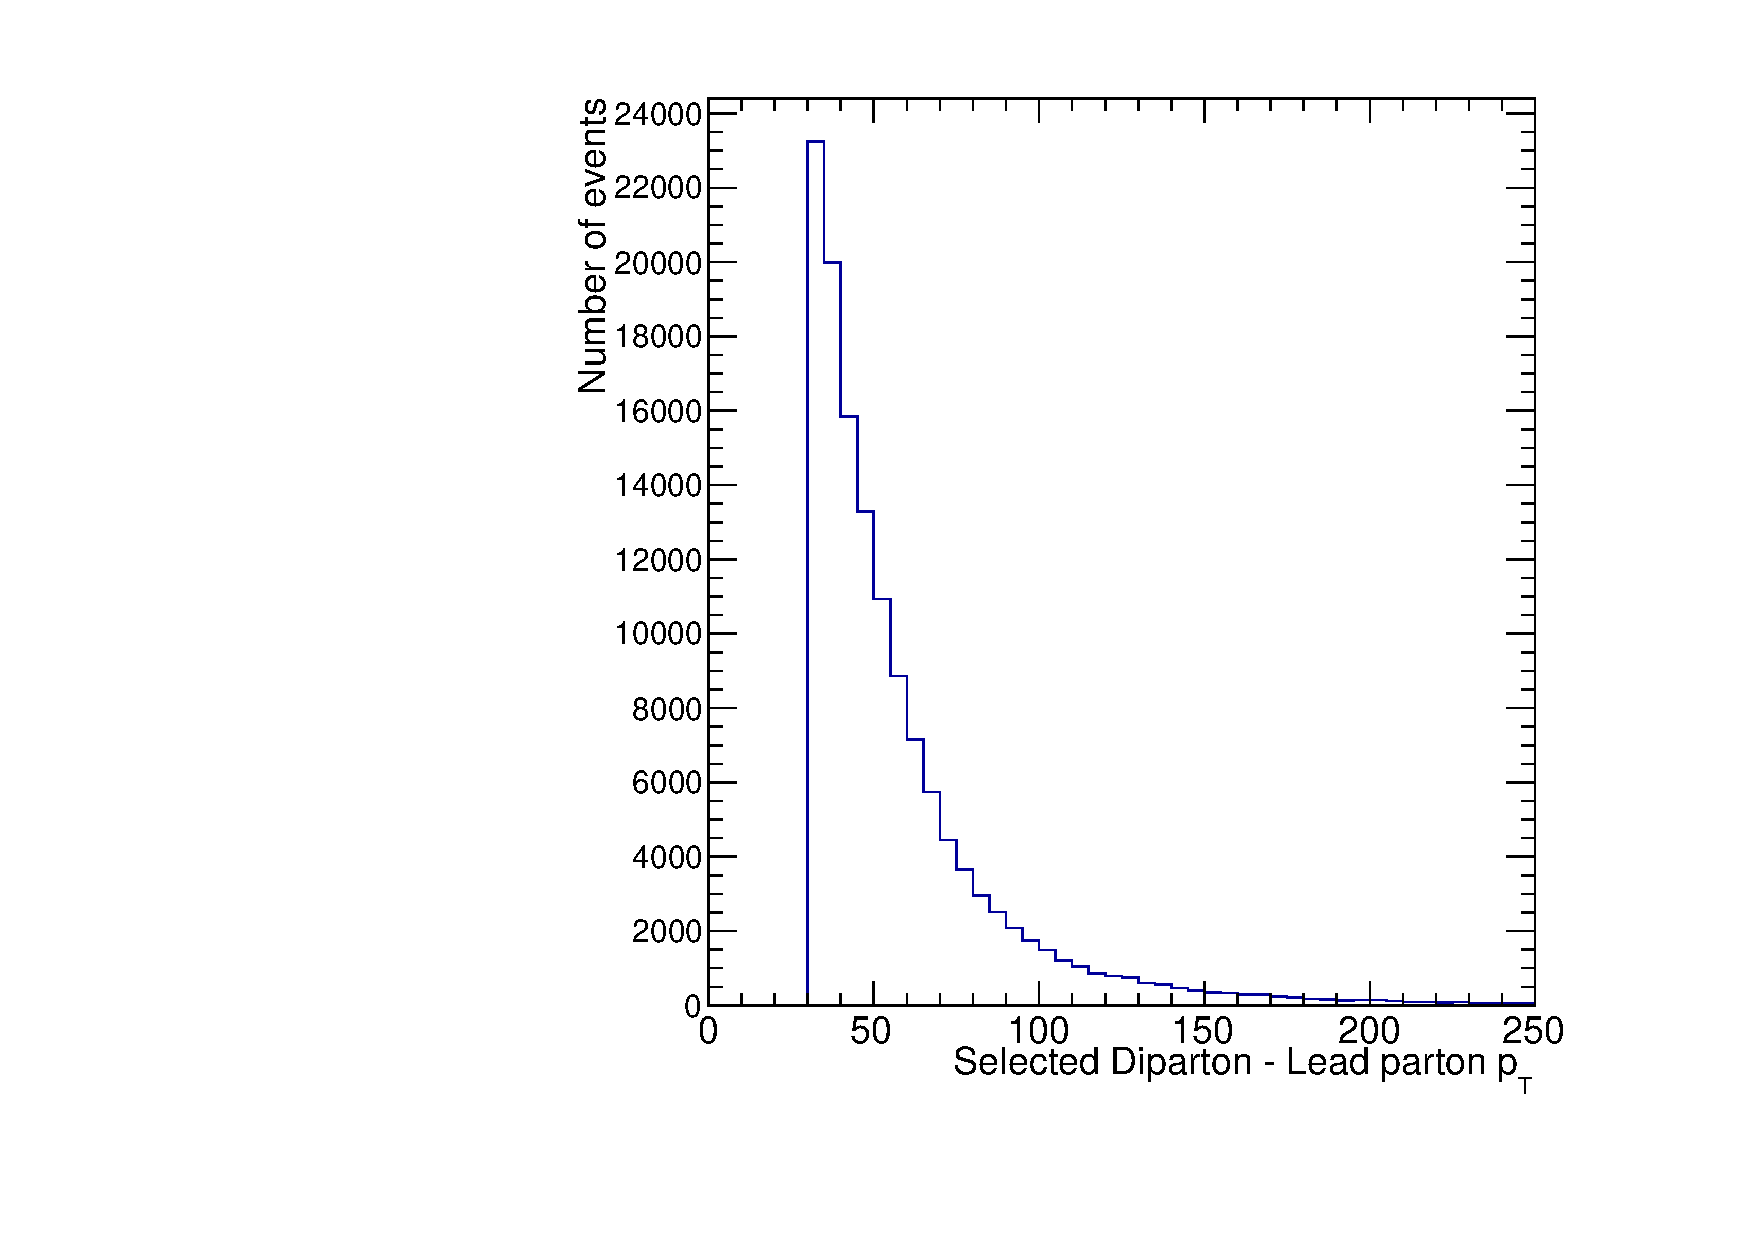
\includegraphics[width=0.40\linewidth]{Chapter07/QCDVBFSamples/PartonFilter/Images/SelDiParton_Parton1_Pt.pdf}}\qquad
\subfloat[][]{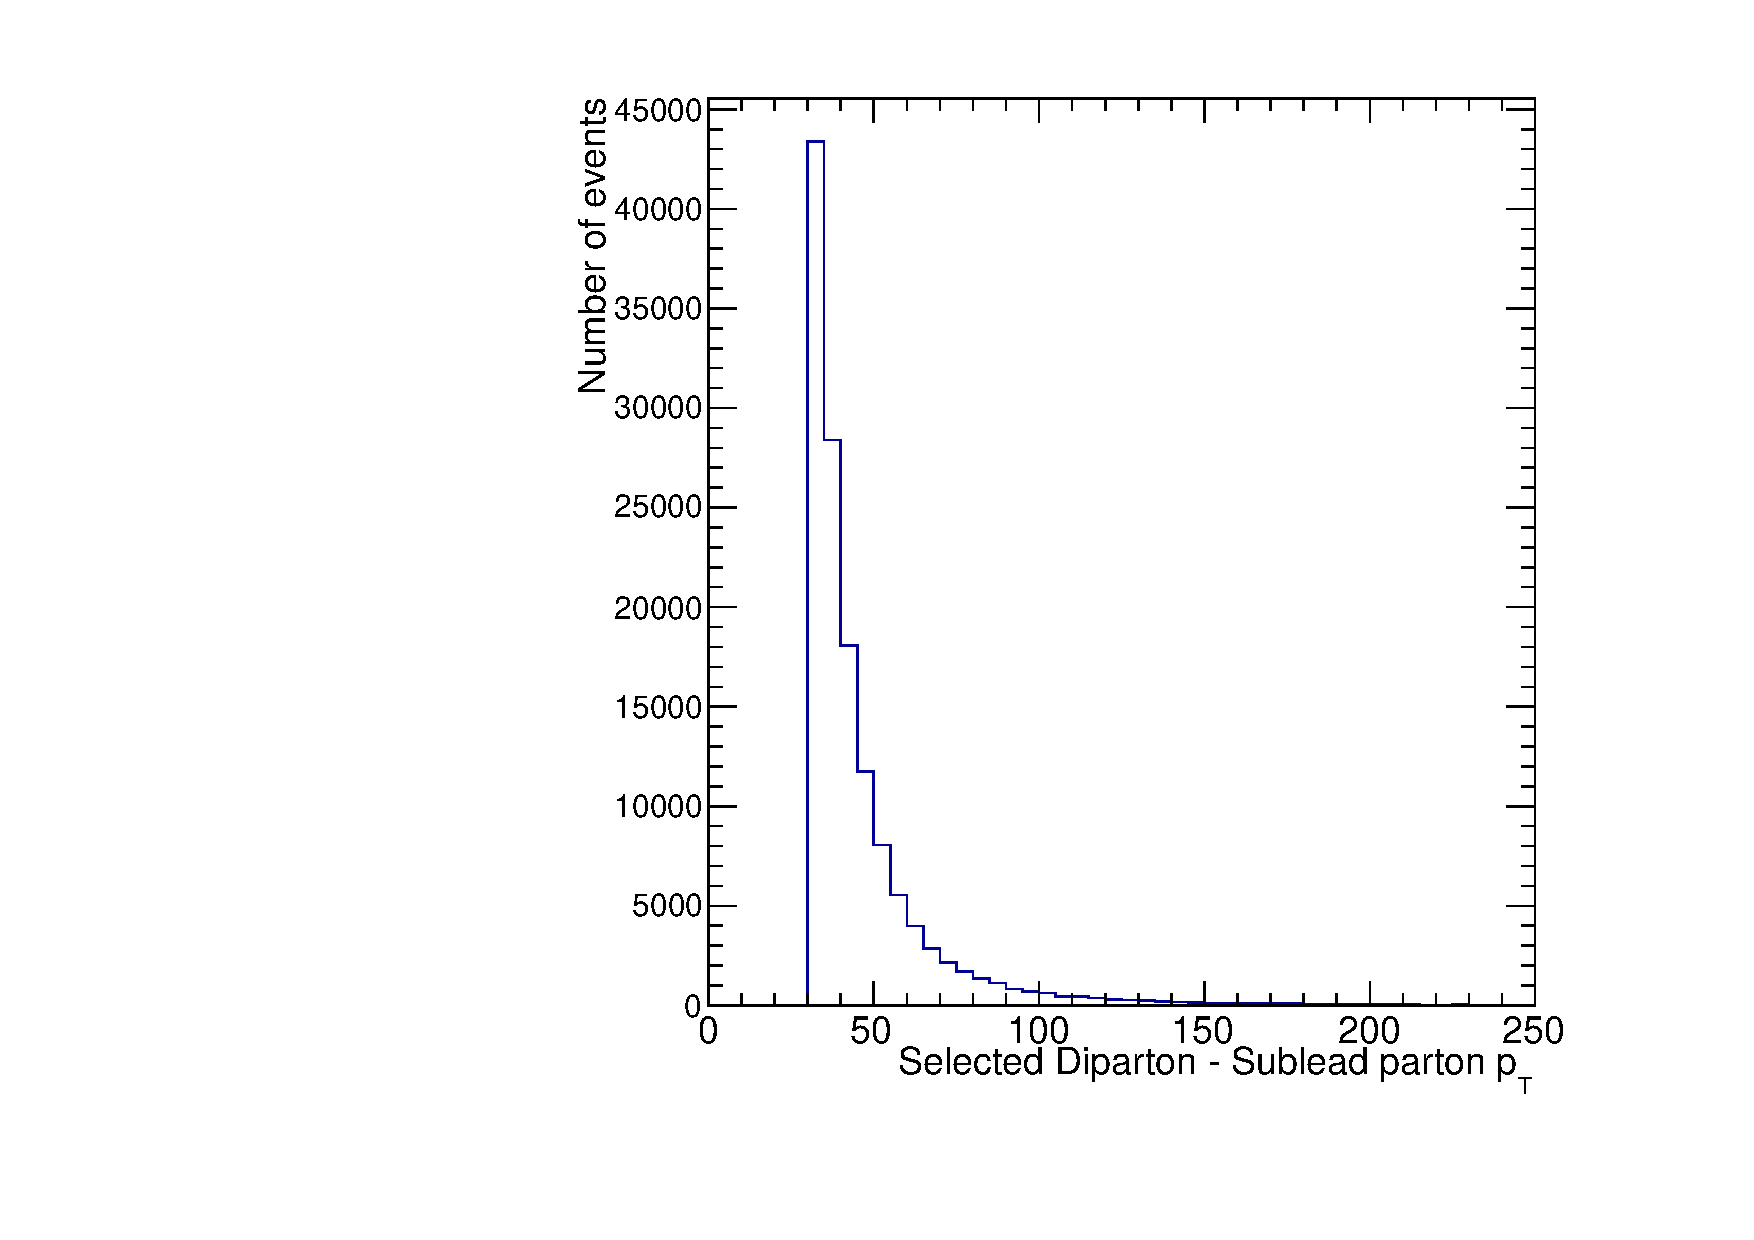
\includegraphics[width=0.40\linewidth]{Chapter07/QCDVBFSamples/PartonFilter/Images/SelDiParton_Parton2_Pt.pdf}}\\
\subfloat[][]{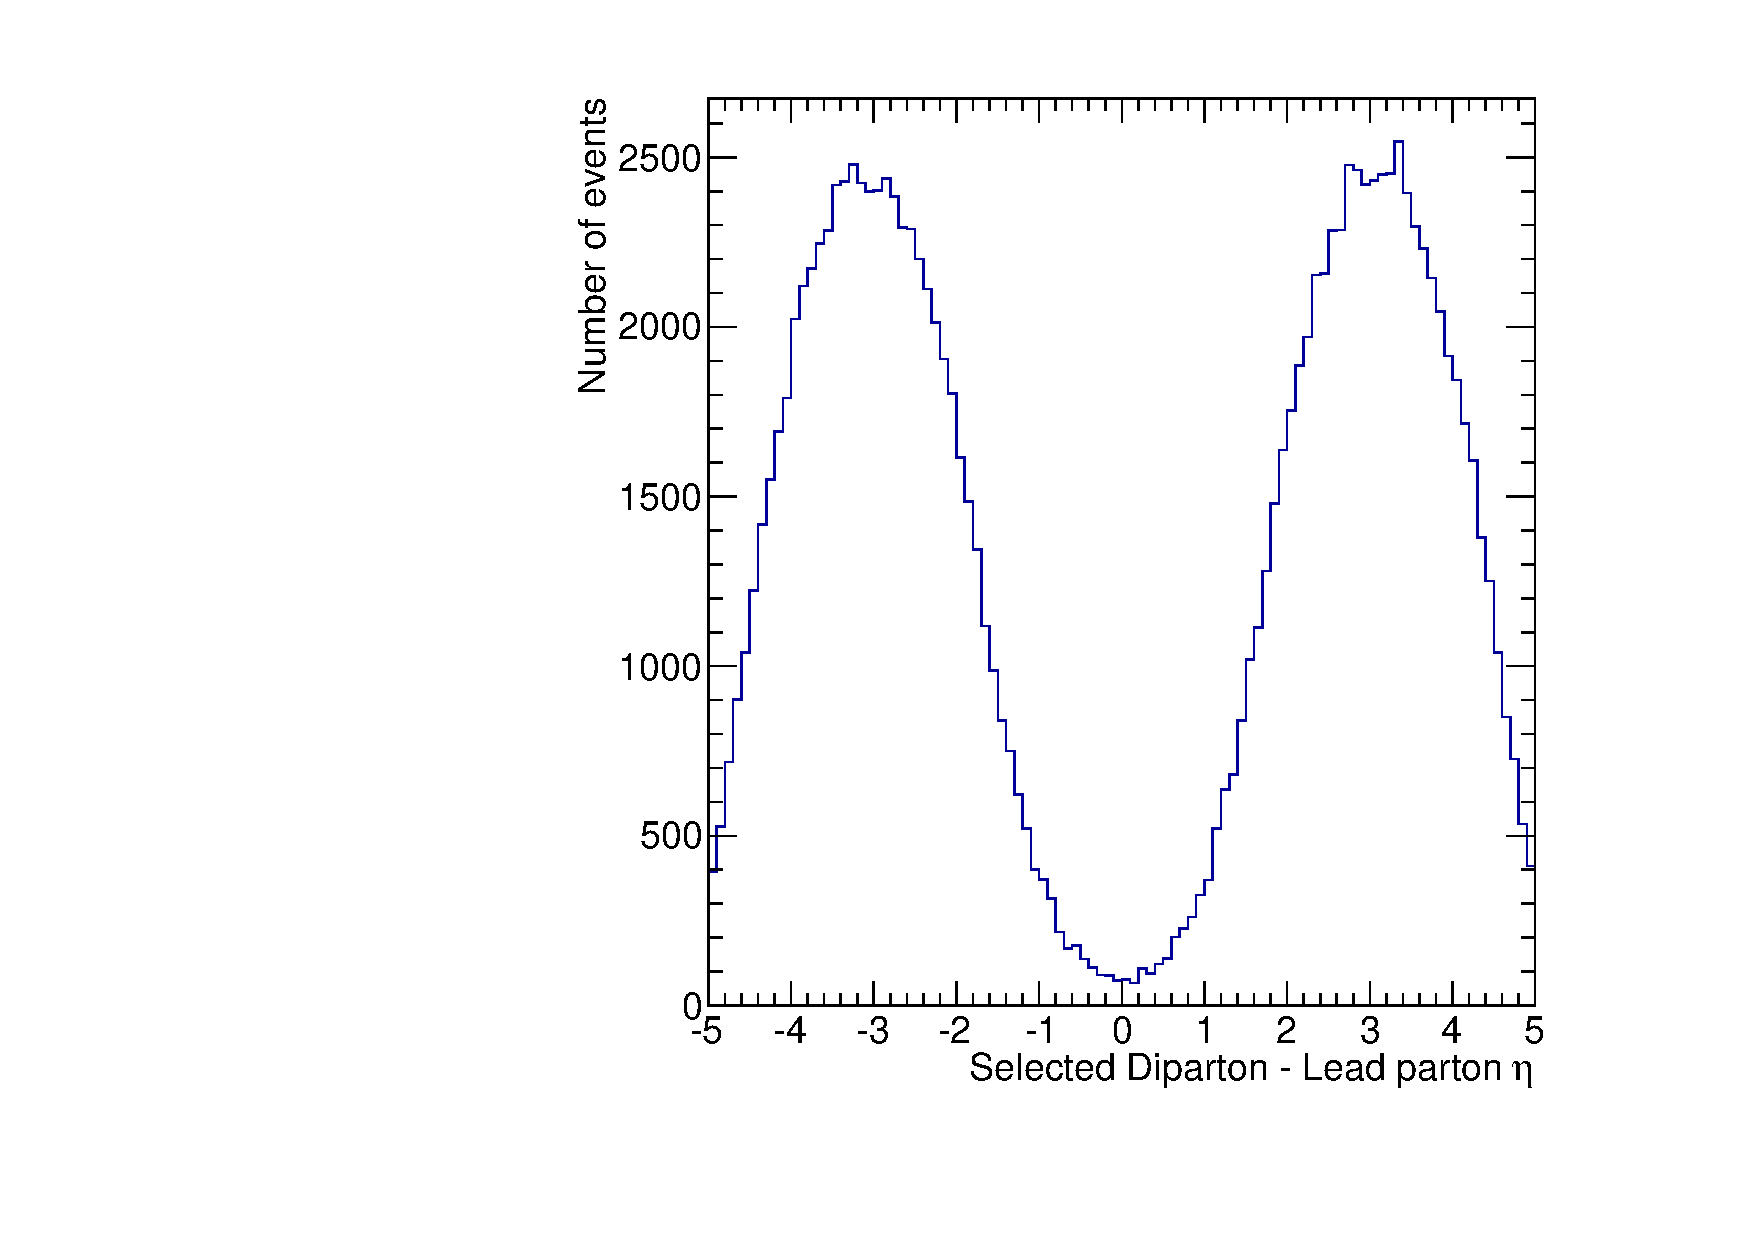
\includegraphics[width=0.40\linewidth]{Chapter07/QCDVBFSamples/PartonFilter/Images/SelDiParton_Parton1_Eta.pdf}}\qquad
\subfloat[][]{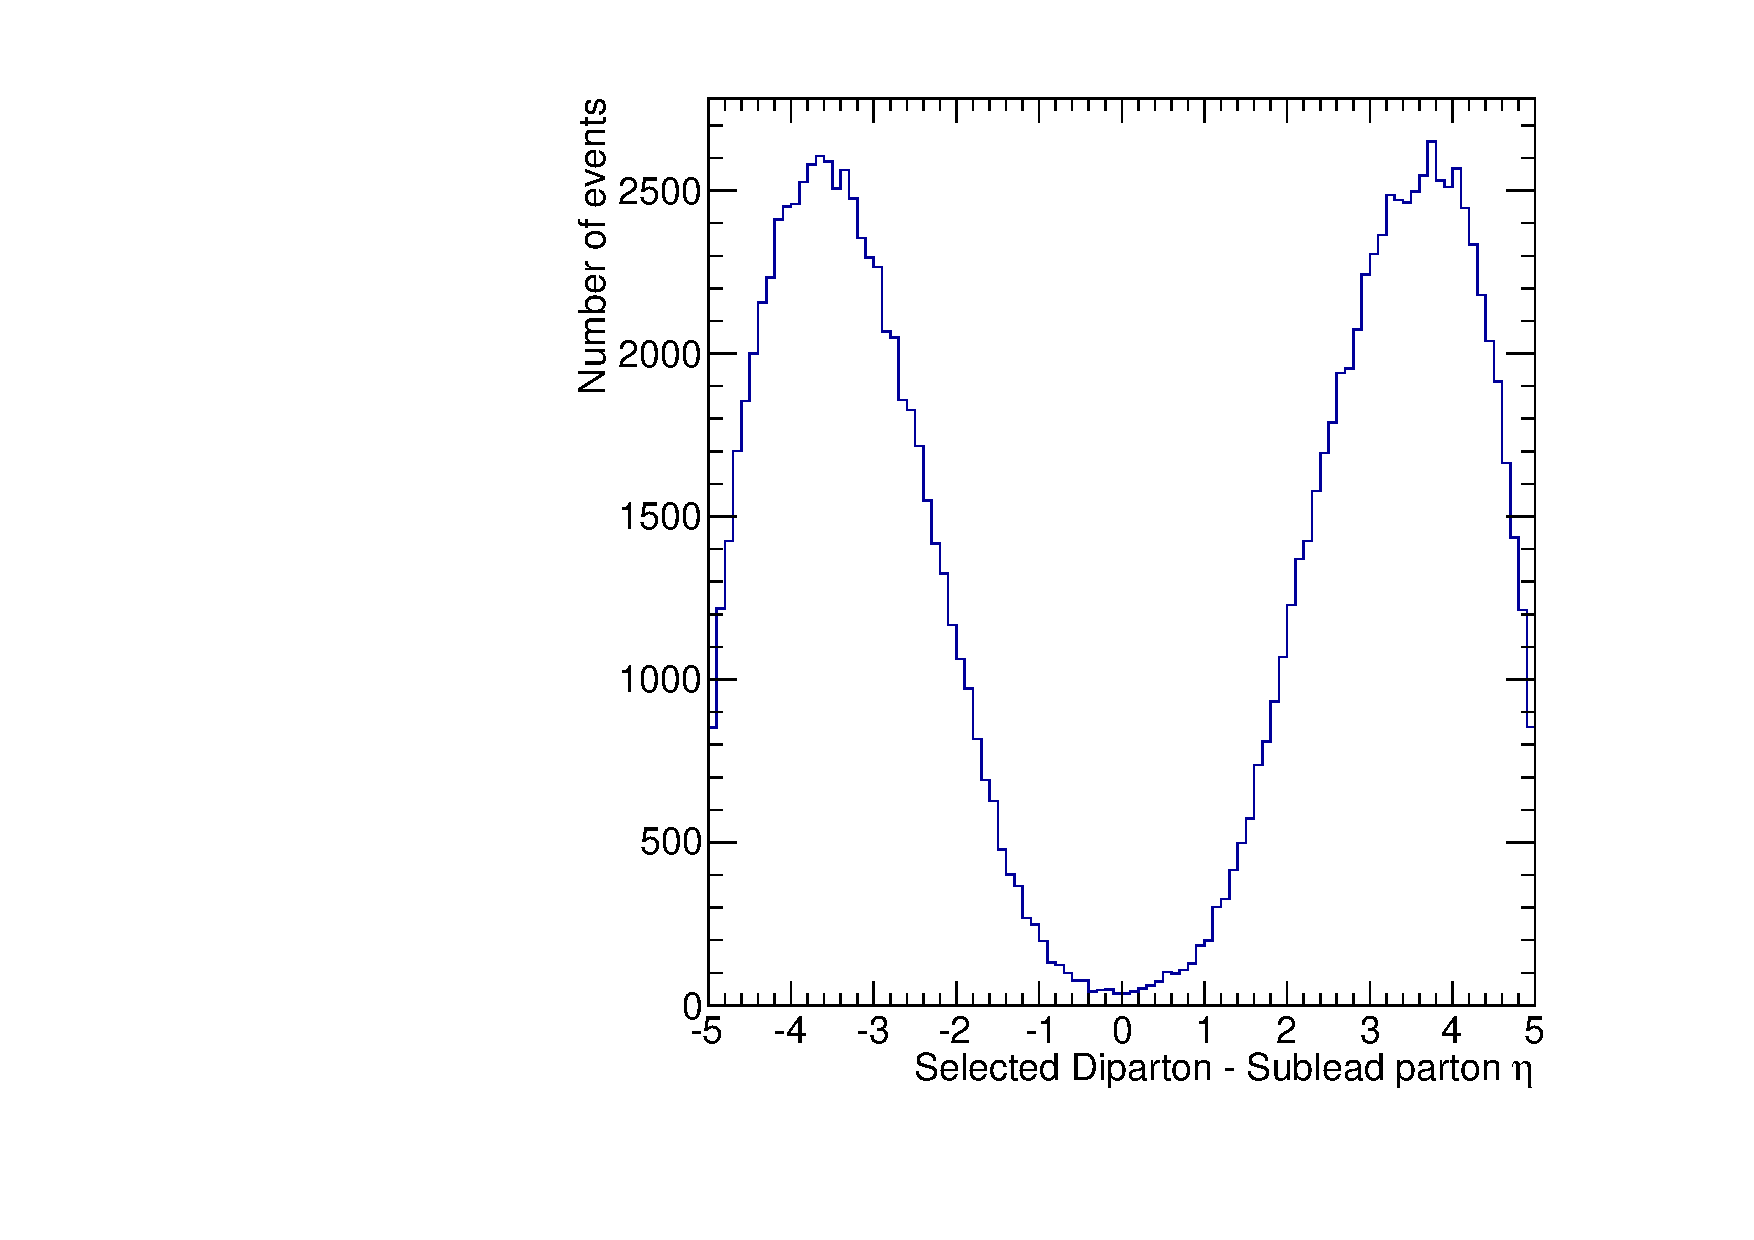
\includegraphics[width=0.40\linewidth]{Chapter07/QCDVBFSamples/PartonFilter/Images/SelDiParton_Parton2_Eta.pdf}}\\
% \subfloat[][]{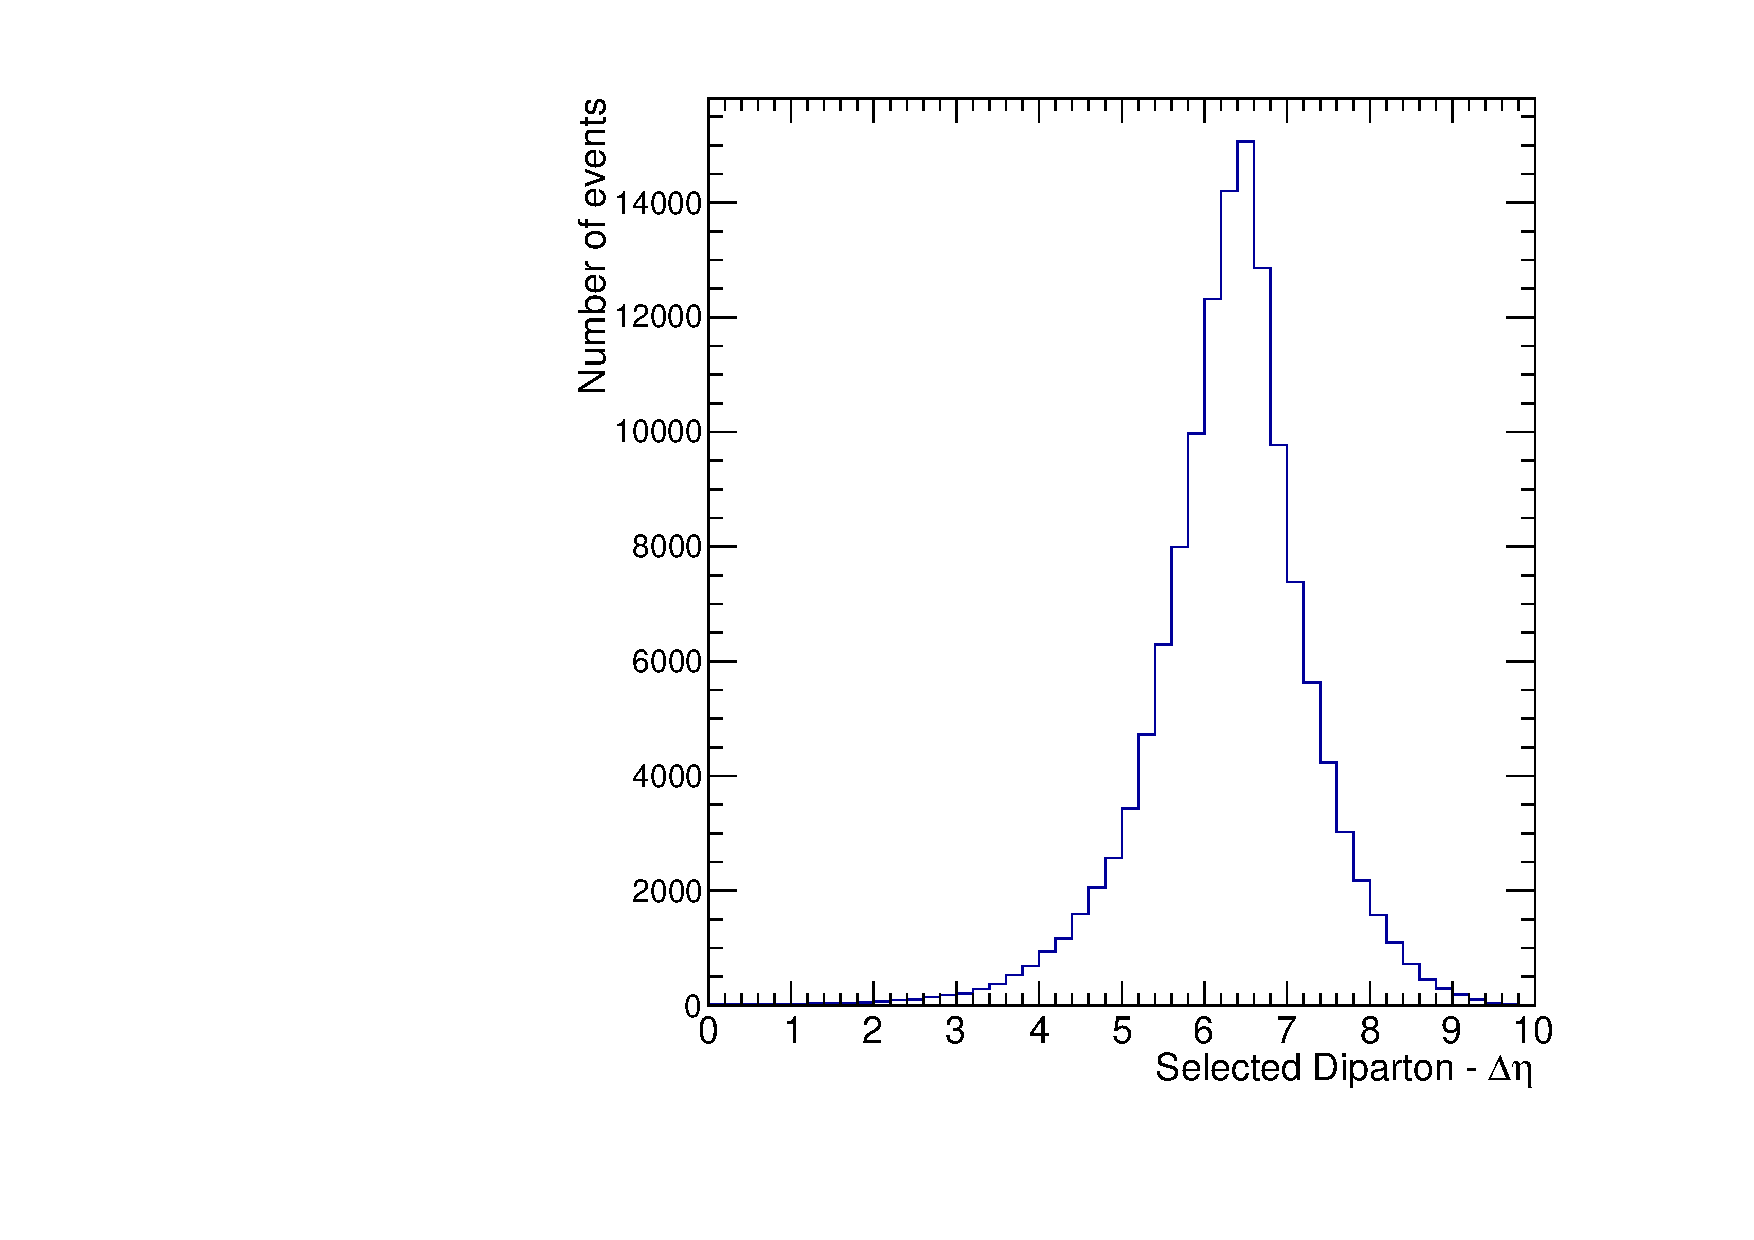
\includegraphics[width=0.45\linewidth]{Chapter07/QCDVBFSamples/PartonFilter/Images/SelDiParton_DEta.pdf}}\qquad
% \subfloat[][]{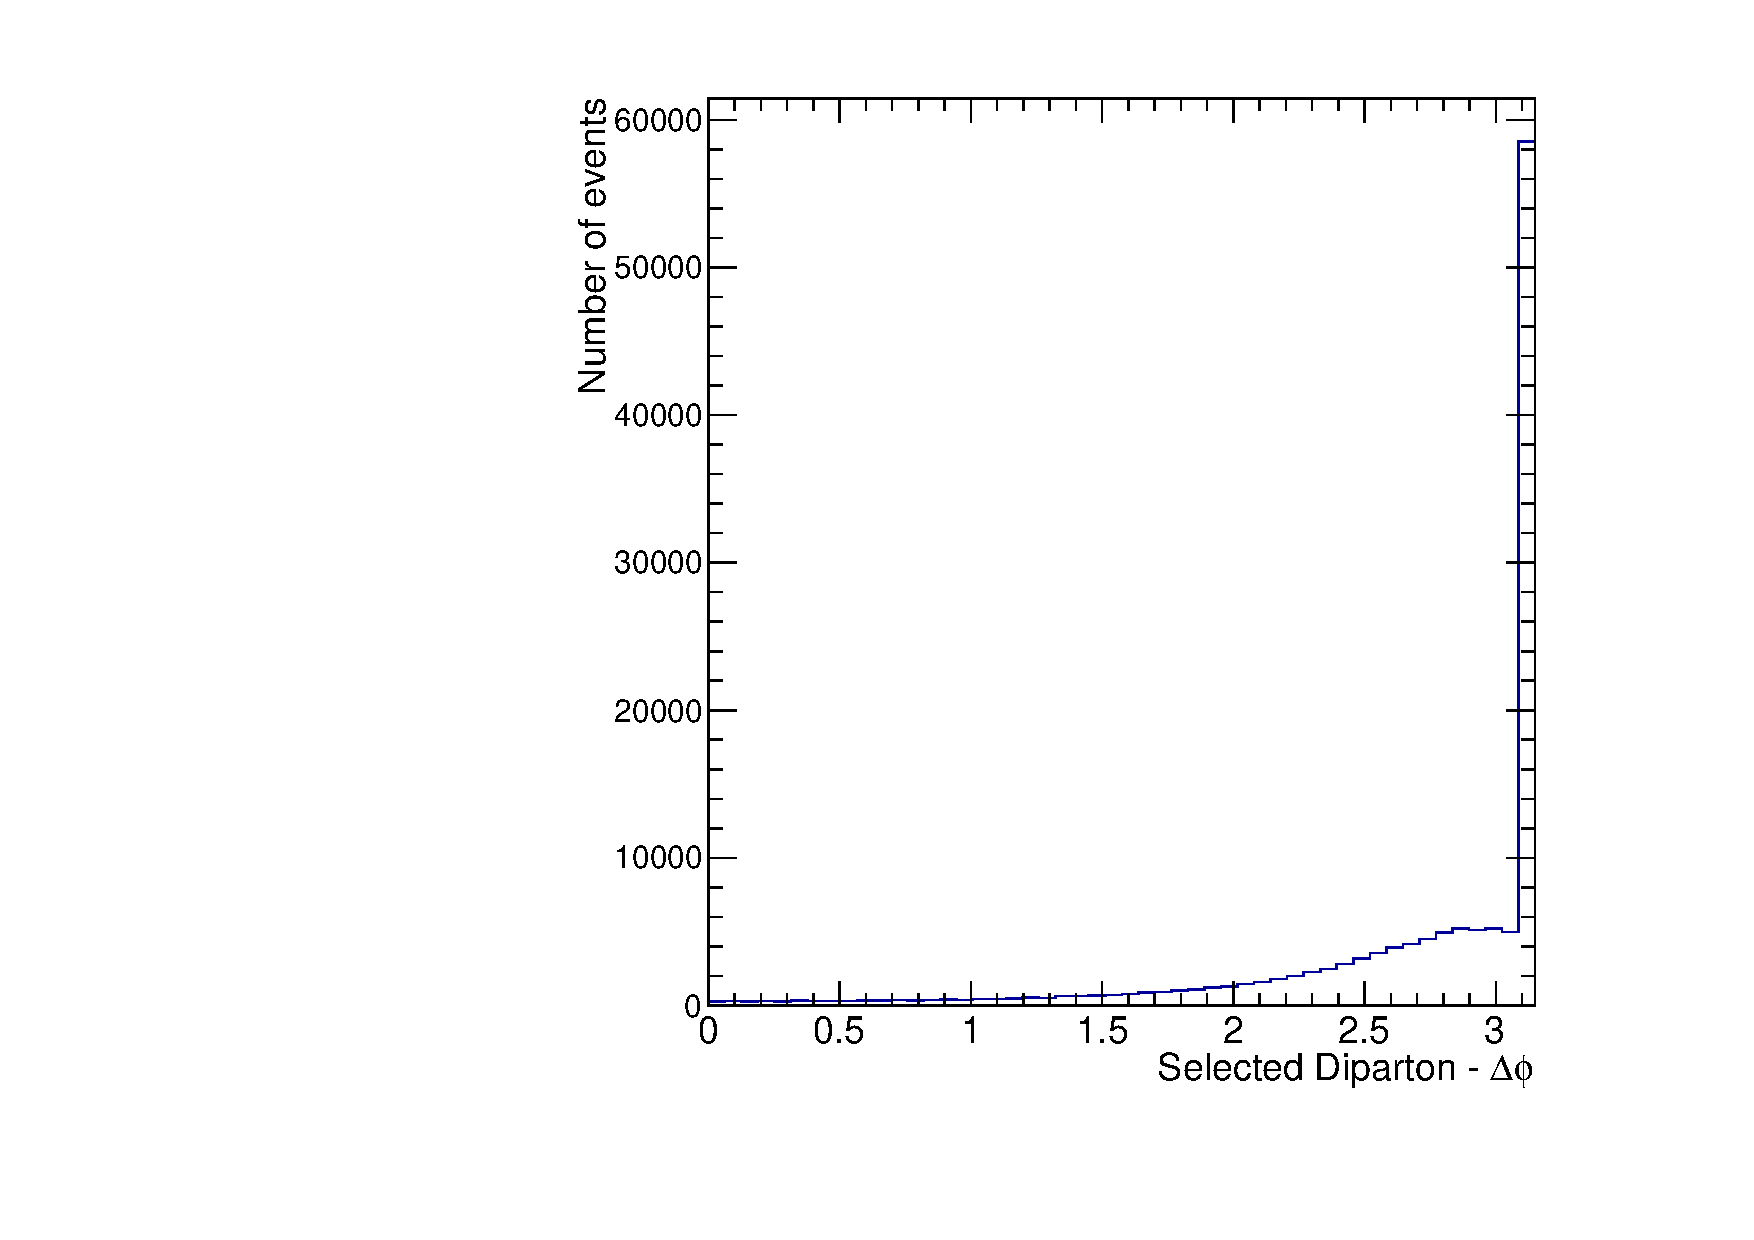
\includegraphics[width=0.45\linewidth]{Chapter07/QCDVBFSamples/PartonFilter/Images/SelDiParton_DPhi.pdf}}\\
\subfloat[][]{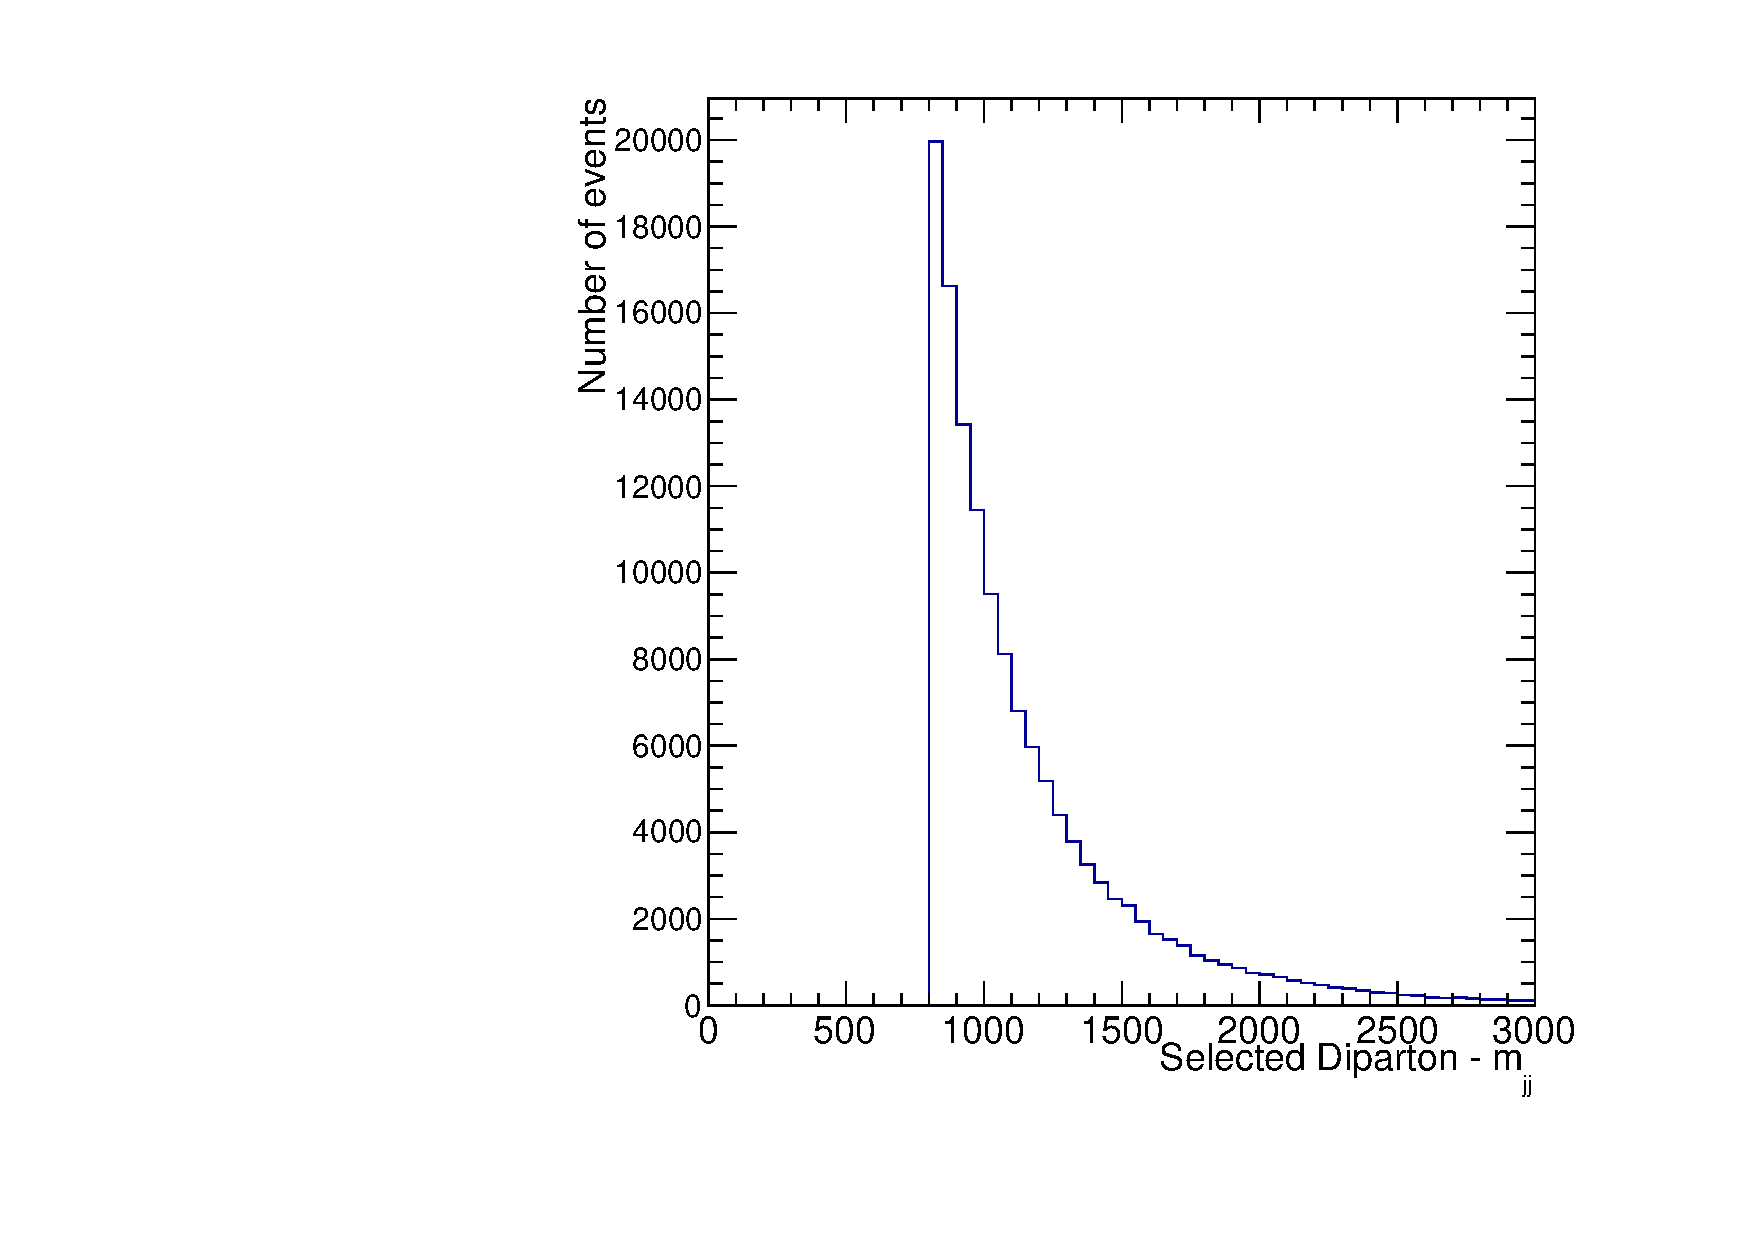
\includegraphics[width=0.40\linewidth]{Chapter07/QCDVBFSamples/PartonFilter/Images/SelDiParton_Mjj.pdf}}\\
\caption[Key variables of events passing the parton level filter]{Parton \pt, $\eta$ and di-parton $m_jj$ distributions for the leading di-parton passing cuts: parton $p_{T}>30\,\GeV$ and $|\eta|<5.0$, di-parton $m_{jj}>800\,\GeV$}
\label{FIGURE:RunIIPreparation_PassPartonFilterDistributions}
\end{figure}

The estimated cross section for this processes and selection is $1.029 \times 10^7 \pm 1.614 \times 10^4 \,\pico\barn$ and we request the production of $1.2 \time 10^{10}$ events. That corresponds to an equivalent luminosity of just over $1.1\,\femto\barn^{-1}$ of equivalent integrated luminosity. 

%%%%%%%%%%%%%%%%%%%%%%%%%%%%%%%%%%%%%%%%%%%%%%%%%%%%%%%%%%%%%%%%%%%%%%%%%%%%%%%%%%%%%%%
%%% SUBSECTION
%%%%%%%%%%%%%%%%%%%%%%%%%%%%%%%%%%%%%%%%%%%%%%%%%%%%%%%%%%%%%%%%%%%%%%%%%%%%%%%%%%%%%%%
\subsection{Hadronization with Pythia 8}
\label{SUBSECTION:RunIIPreparation_HadronizationWithPythia8}

%Status: DONE

The parton level events that have passed the initial filter now have to be hadronized. Similarly to other samples produced in the \gls{CMS} we have chosen Pythia 8 for this task. As described in section \ref{SUBSECTION:RunIIPreparation_MonteCarloSampleSimulation} when using a \gls{ME} generator with a shower generator we need to filter the overlapping phase-space. As for recommendation of the \gls{CMS} generator group we used the MLM scheme with the same parameters used for the production of previous official samples. The results of the hadronization process are summarized in table \ref{TABLE:RunIIPreparation_Pythia8HadronizationResults}.

\begin{table}[!htp]
\centering

\resizebox{1.0\textwidth}{!}{
\begin{tabular}{|c|c|c|c|c|c|}
\hline
                          & \multicolumn{3}{c|}{Events}      & \multicolumn{2}{c|}{Cross Section [pb]}                \\
\hline
Process                   &  Tried  & Passed & accepted [\%]  & Before                    & After                     \\
\hline\hline 
$p p \rightarrow j j$     &  231789 &  54291 & $23.4 \pm 1.01$ & $1.675 \times 10^6 \pm 4.536 \times 10^3$ & $3.924 \times 10^5 \pm 1.817 \times 10^3$ \\
$p p \rightarrow j j j$   &  502287 &  36250 & $ 7.2 \pm 0.03$ & $3.622 \times 10^6 \pm 9.809 \times 10^3$ & $2.614 \times 10^5 \pm 1.500 \times 10^3$ \\
$p p \rightarrow j j j j$ &  692600 &  44299 & $ 6.4 \pm 0.03$ & $4.972 \times 10^6 \pm 1.346 \times 10^4$ & $3.180 \times 10^5 \pm 1.697 \times 10^3$ \\
\hline\hline
Total                     & 1426676 & 134840 & $9.45 \pm 0.03$ & $1.027 \times 10^7 \pm 1.727 \times 10^4$ & $9.718 \times 10^5 \pm 2.903 \times 10^3$ \\
\hline
\end{tabular}
}
\caption{Summary of the results of the Hadronization with Pythia 8 of 1.4M MadGraph events passing the parton level filter.}
\label{TABLE:RunIIPreparation_Pythia8HadronizationResults}
\end{table}

% --------------------------------------------------------------------------------------------------------------------------------------------------------------------------
% Process and cross-section statistics
% --------------------------------------------------------------------------------------------------------------------------------------------------------------------------
% Process         xsec_before [pb]                passed  nposw   nnegw   tried   nposw   nnegw   xsec_match [pb]                 accepted [%]     event_eff [%]
% 0               1.675e+06 +/- 4.536e+03         54291   54291   0       231789  231789  0       3.924e+05 +/- 1.817e+03         23.4 +/- 0.1    23.4 +/- 0.1       1.0052431
% 1               3.622e+06 +/- 9.809e+03         36250   36250   0       502287  502287  0       2.614e+05 +/- 1.500e+03          7.2 +/- 0.0     7.2 +/- 0.0       0.037905486
% 2               4.972e+06 +/- 1.346e+04         44299   44299   0       692600  692600  0       3.180e+05 +/- 1.697e+03          6.4 +/- 0.0     6.4 +/- 0.0       0.030388865
% --------------------------------------------------------------------------------------------------------------------------------------------------------------------------
% Total           1.027e+07 +/- 1.727e+04         134840  134840  0       1426676 1426676 0       9.718e+05 +/- 2.903e+03          9.5 +/- 0.0     9.5 +/- 0.0
% --------------------------------------------------------------------------------------------------------------------------------------------------------------------------


Efficiency of the post hadronization event matching has been estimated of $9.45\% \pm 0.03\%$, leading to an sample cross section of $9.718 \times 10^5 \pm 2.903 \times 10^3\,\pico\barn$. The lower matching efficiency in the 3 and 4 jets final states is due to the absence of a restriction on minimum jet \pt on any additional jets to the dijet passing the parton level cuts. This jets, if low enough on energy will hardly be clusters into a jet and therefore cannot be match to its seed parton.

%%%%%%%%%%%%%%%%%%%%%%%%%%%%%%%%%%%%%%%%%%%%%%%%%%%%%%%%%%%%%%%%%%%%%%%%%%%%%%%%%%%%%%%
%%% SUBSECTION
%%%%%%%%%%%%%%%%%%%%%%%%%%%%%%%%%%%%%%%%%%%%%%%%%%%%%%%%%%%%%%%%%%%%%%%%%%%%%%%%%%%%%%%
\subsection{Generator level cuts}
\label{SUBSECTION:RunIIPreparation_GeneratorLevelCuts}

%Status: DONE

After hadronization we cluster the outgoing stable particles with the anti-$k_T$ algorithm with $\Delta R<0.4$ while ignoring muons. The reason to ignore muons is that \gls{CMS} muon detector coverage only goes up to $|\eta|<2.4$ so all muons outside this region will not be seen by the experiment and therefore will not be clustered into jets. Most of our signal like events will have at least one jet in the region $|\eta|>2.4$. 

We start by making an initial selection of the events with at least one generator level dijet passing $\Delta\eta > 3.0$, $m_{jj} > 1000\,\GeV$ where both jets pass $\pt > 40\,\GeV$ and $|\eta|<4.8$. The events passing this cuts are split into two sub-samples. Sub-sample A will have the events where the selected dijet passes $\Delta\phi<=2.15$ and sub-sample B where at least on dijet passing all initial conditions and an inverted $\Delta\phi$ cut. Plots over all the relevant variable before the $\Delta\phi$ cut and for the leading dijet passing the cuts can be found in figure \ref{FIGURE:RunIIPreparation_PassGeneratorFilterDistributions1} and \ref{FIGURE:RunIIPreparation_PassGeneratorFilterDistributions2}.

\begin{figure}[!htp]%
\centering
\subfloat[][]{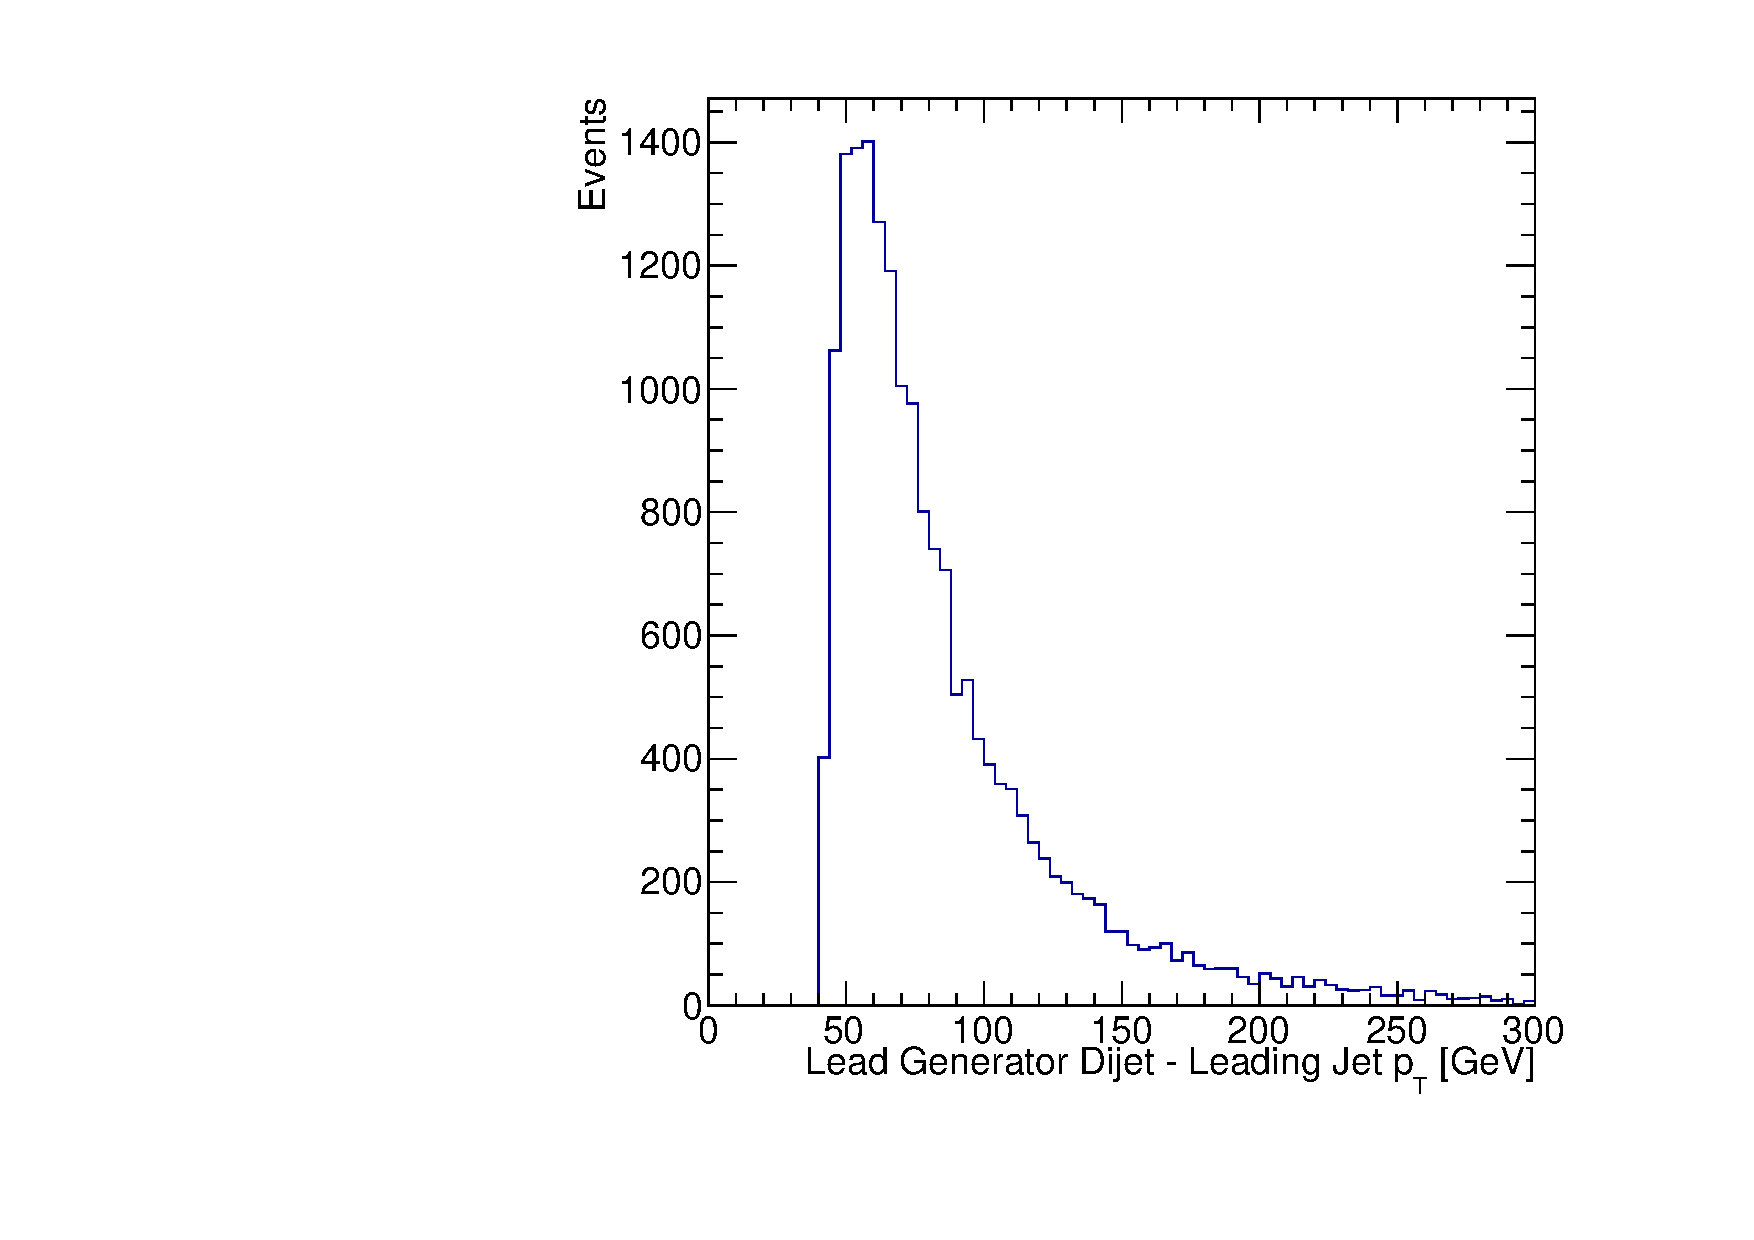
\includegraphics[width=0.40\linewidth]{Chapter07/QCDVBFSamples/GeneratorFilter/Pt40_Eta4p8_DEta3p0_Mjj1000/Images/LeadDijet_Jet0_Pt.pdf}}\qquad
\subfloat[][]{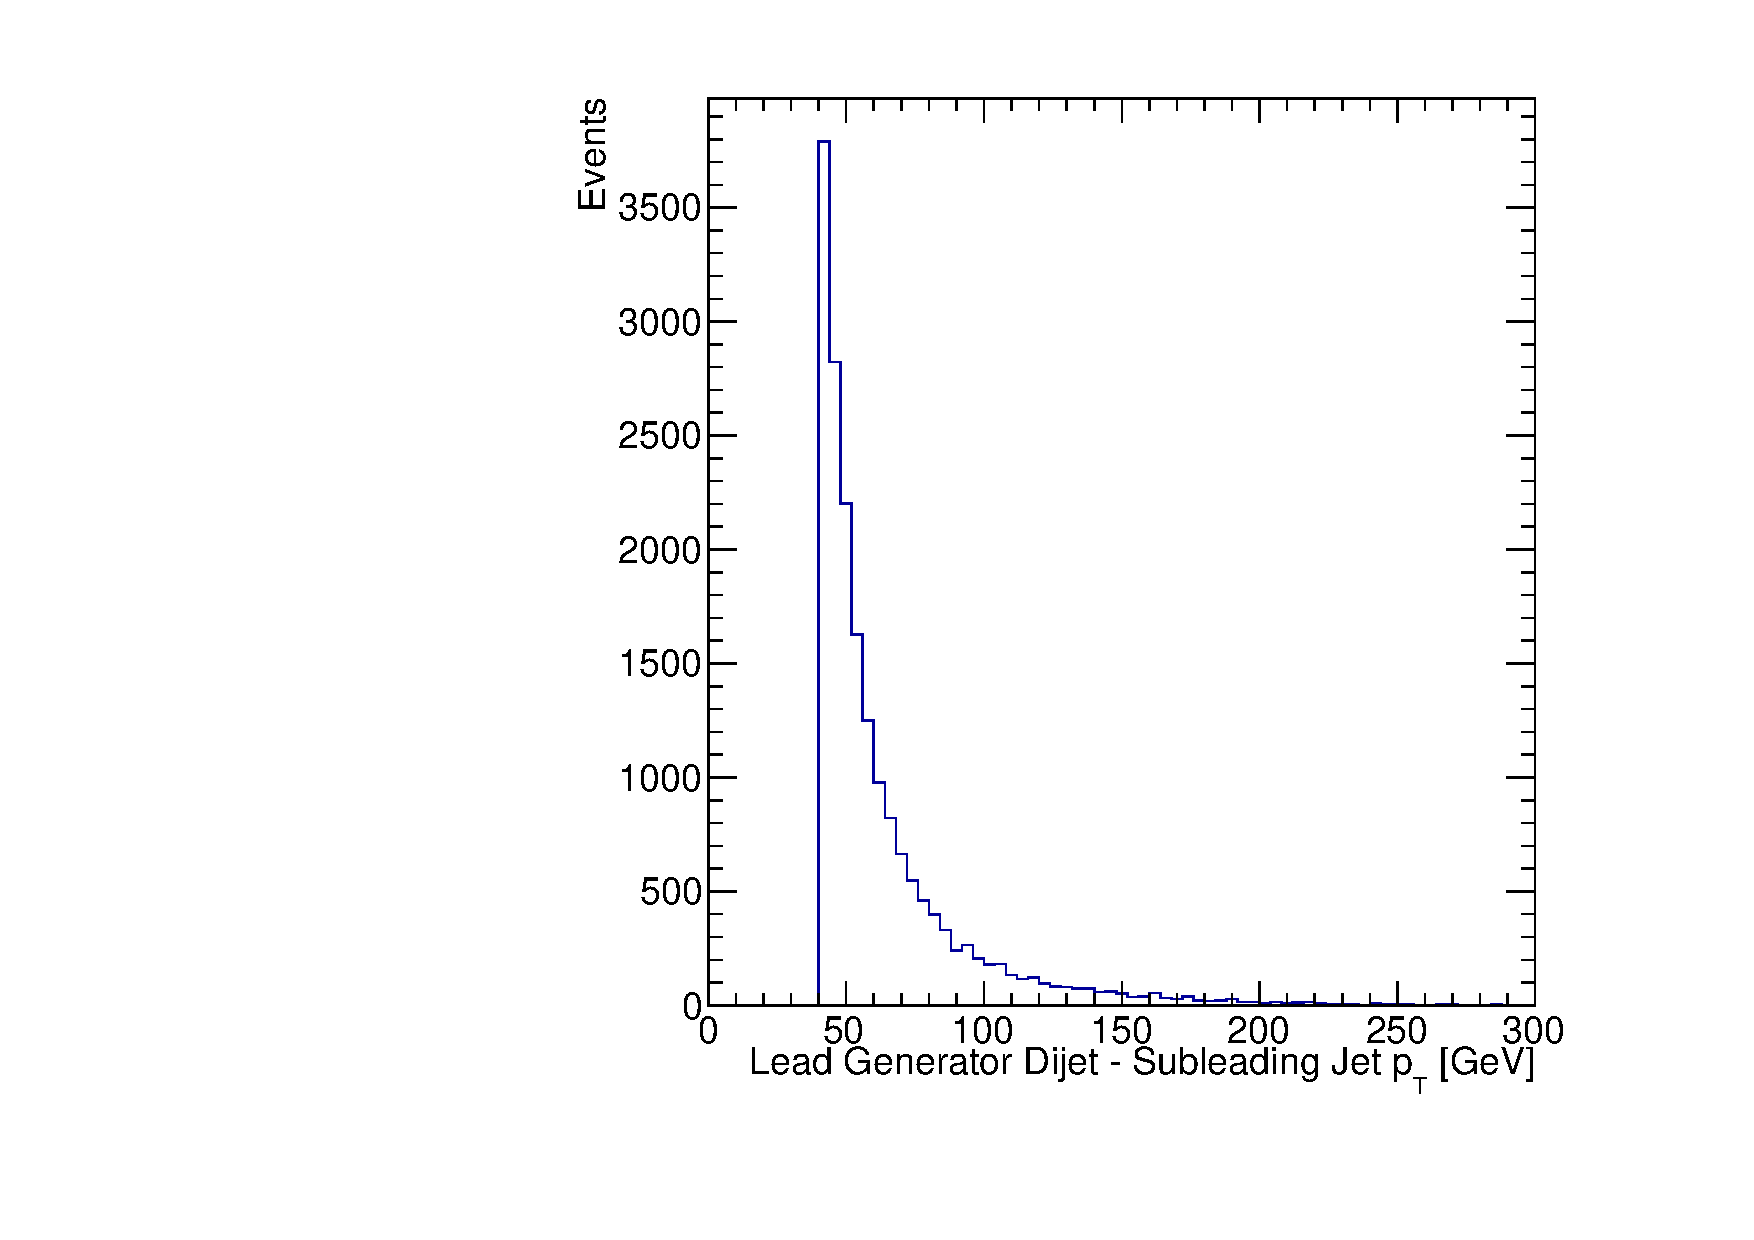
\includegraphics[width=0.40\linewidth]{Chapter07/QCDVBFSamples/GeneratorFilter/Pt40_Eta4p8_DEta3p0_Mjj1000/Images/LeadDijet_Jet1_Pt.pdf}}\\
\subfloat[][]{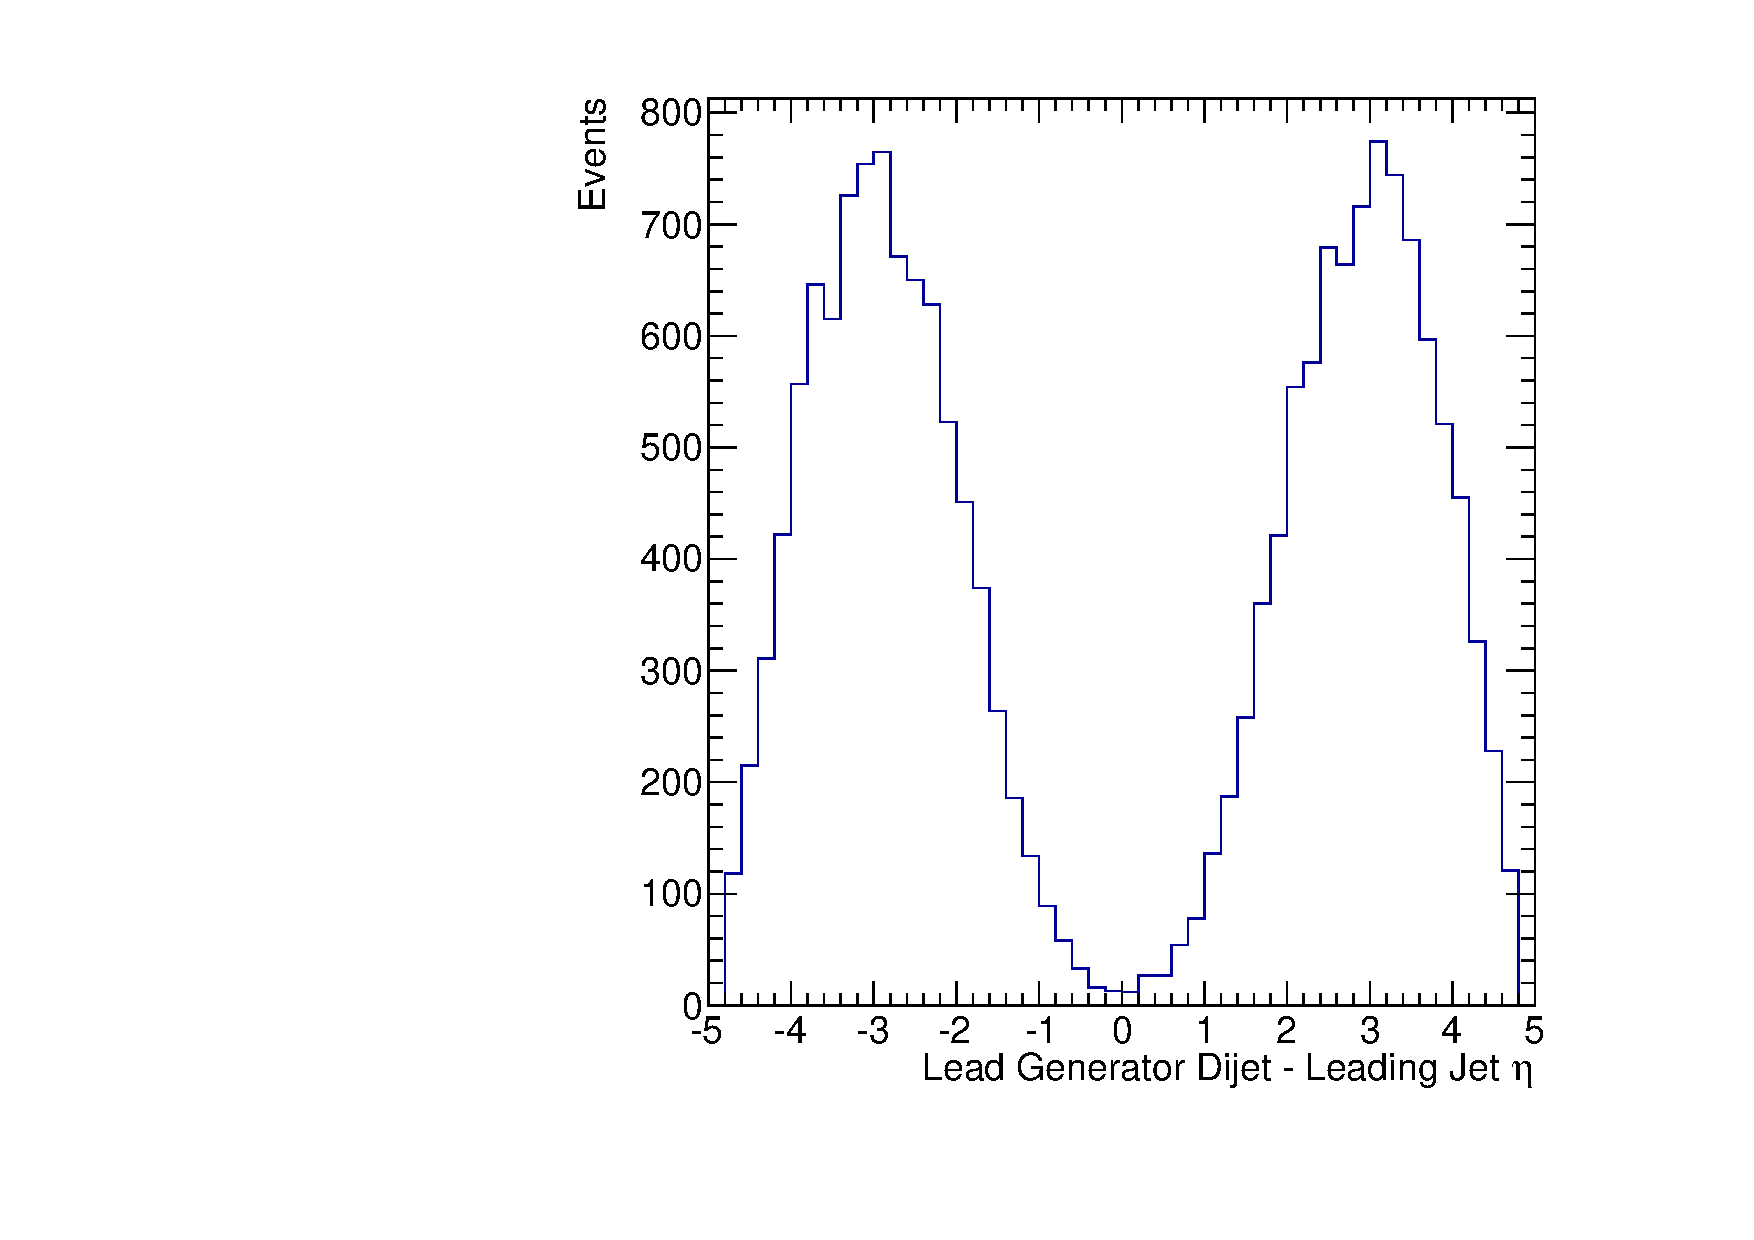
\includegraphics[width=0.40\linewidth]{Chapter07/QCDVBFSamples/GeneratorFilter/Pt40_Eta4p8_DEta3p0_Mjj1000/Images/LeadDijet_Jet0_Eta.pdf}}\qquad
\subfloat[][]{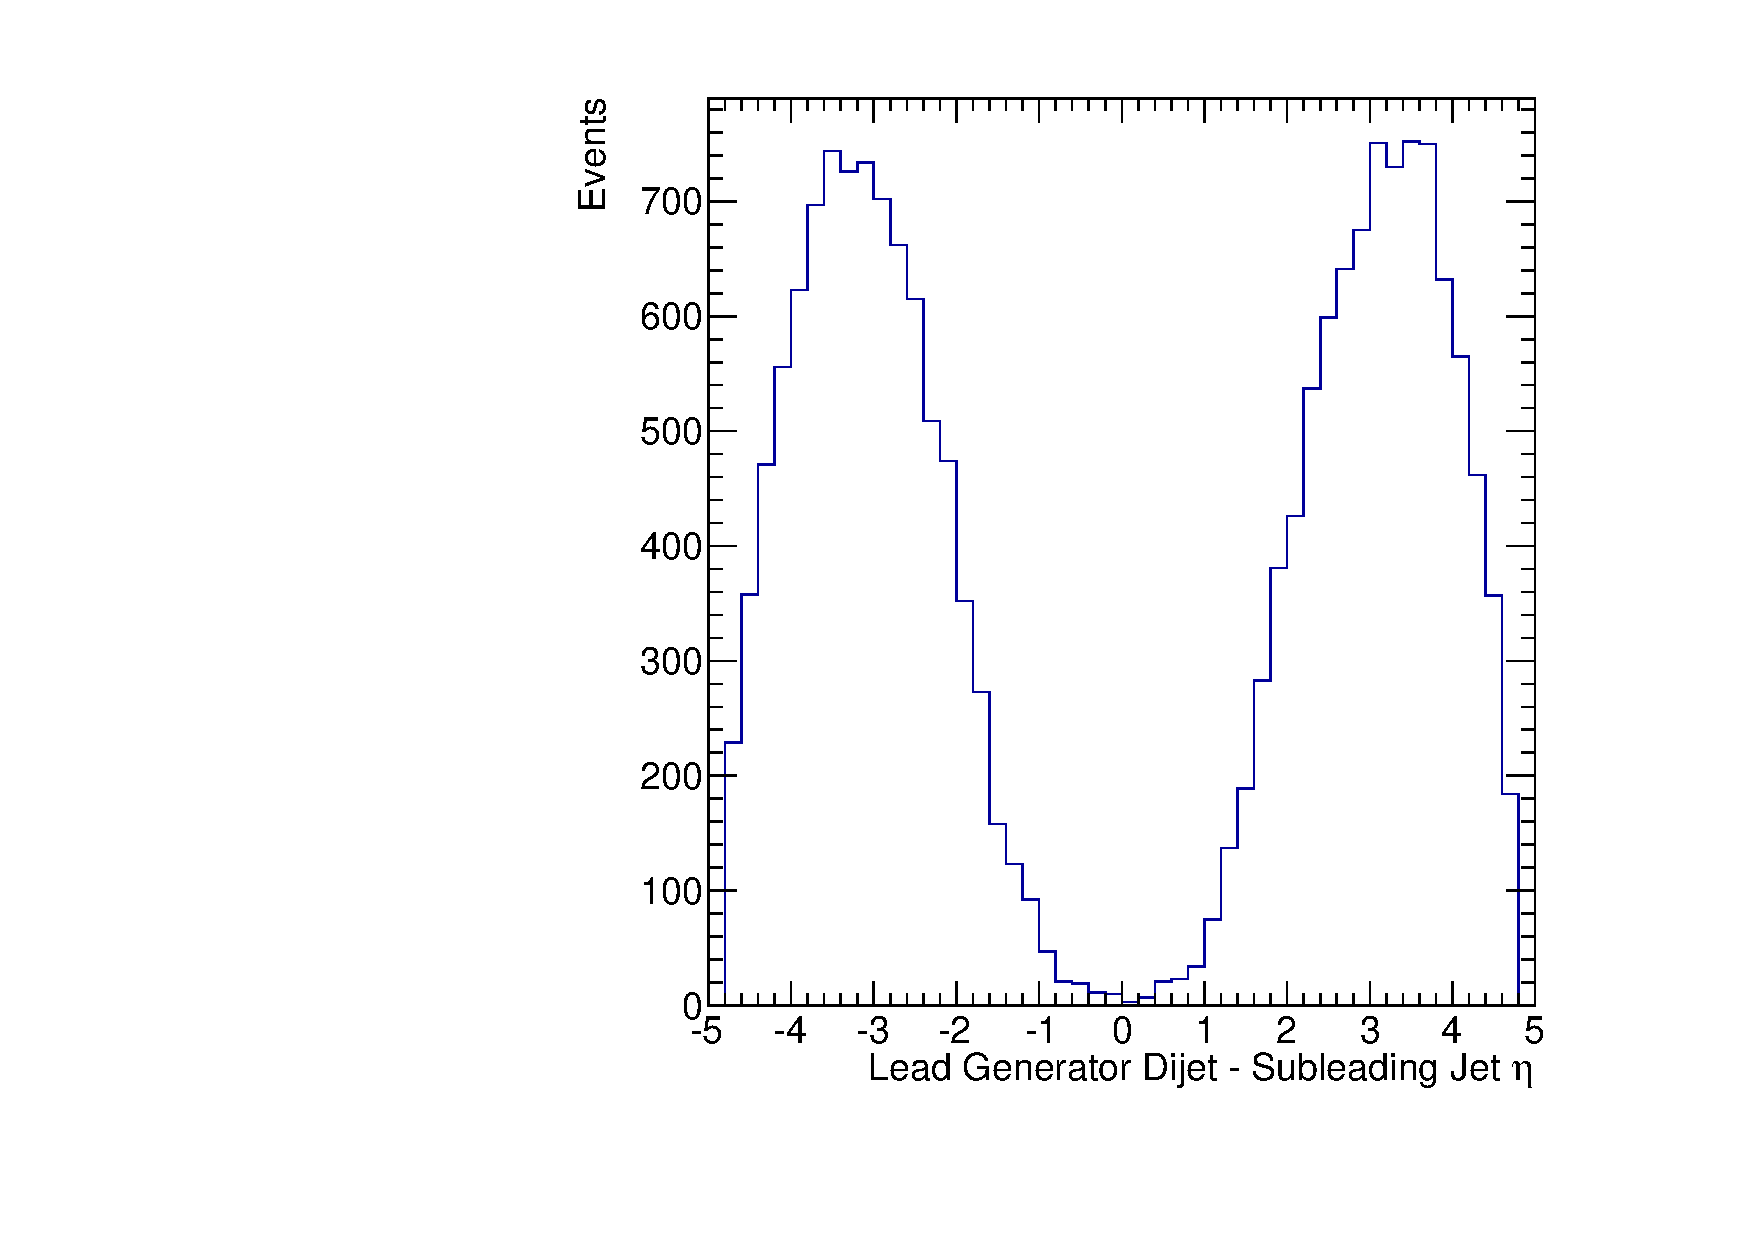
\includegraphics[width=0.40\linewidth]{Chapter07/QCDVBFSamples/GeneratorFilter/Pt40_Eta4p8_DEta3p0_Mjj1000/Images/LeadDijet_Jet1_Eta.pdf}}\\
\caption{Relevant distributions for the two jets comprising the the leading dijet passing a generator filter requiring at least one dijet with $\Delta\eta>3.0$ and $m_{jj}>1000\,\GeV$ where the jets have $\pt>40\,\GeV$ and $|\eta|<4.8$}
\label{FIGURE:RunIIPreparation_PassGeneratorFilterDistributions1}
\end{figure}

All the distributions show the expected features of the generator level filter cuts. As expected the peak of the $\Delta\phi$ distribution is at \pi when the 2 jets are back to back, but a tail of events is visible down to zero. A similar shape was observed in the Run I analysis before applying a cut on $min(\Delta\phi(jets,MET))$ in QCD dominated regions.

\begin{figure}[!htp]%
\centering
\subfloat[][]{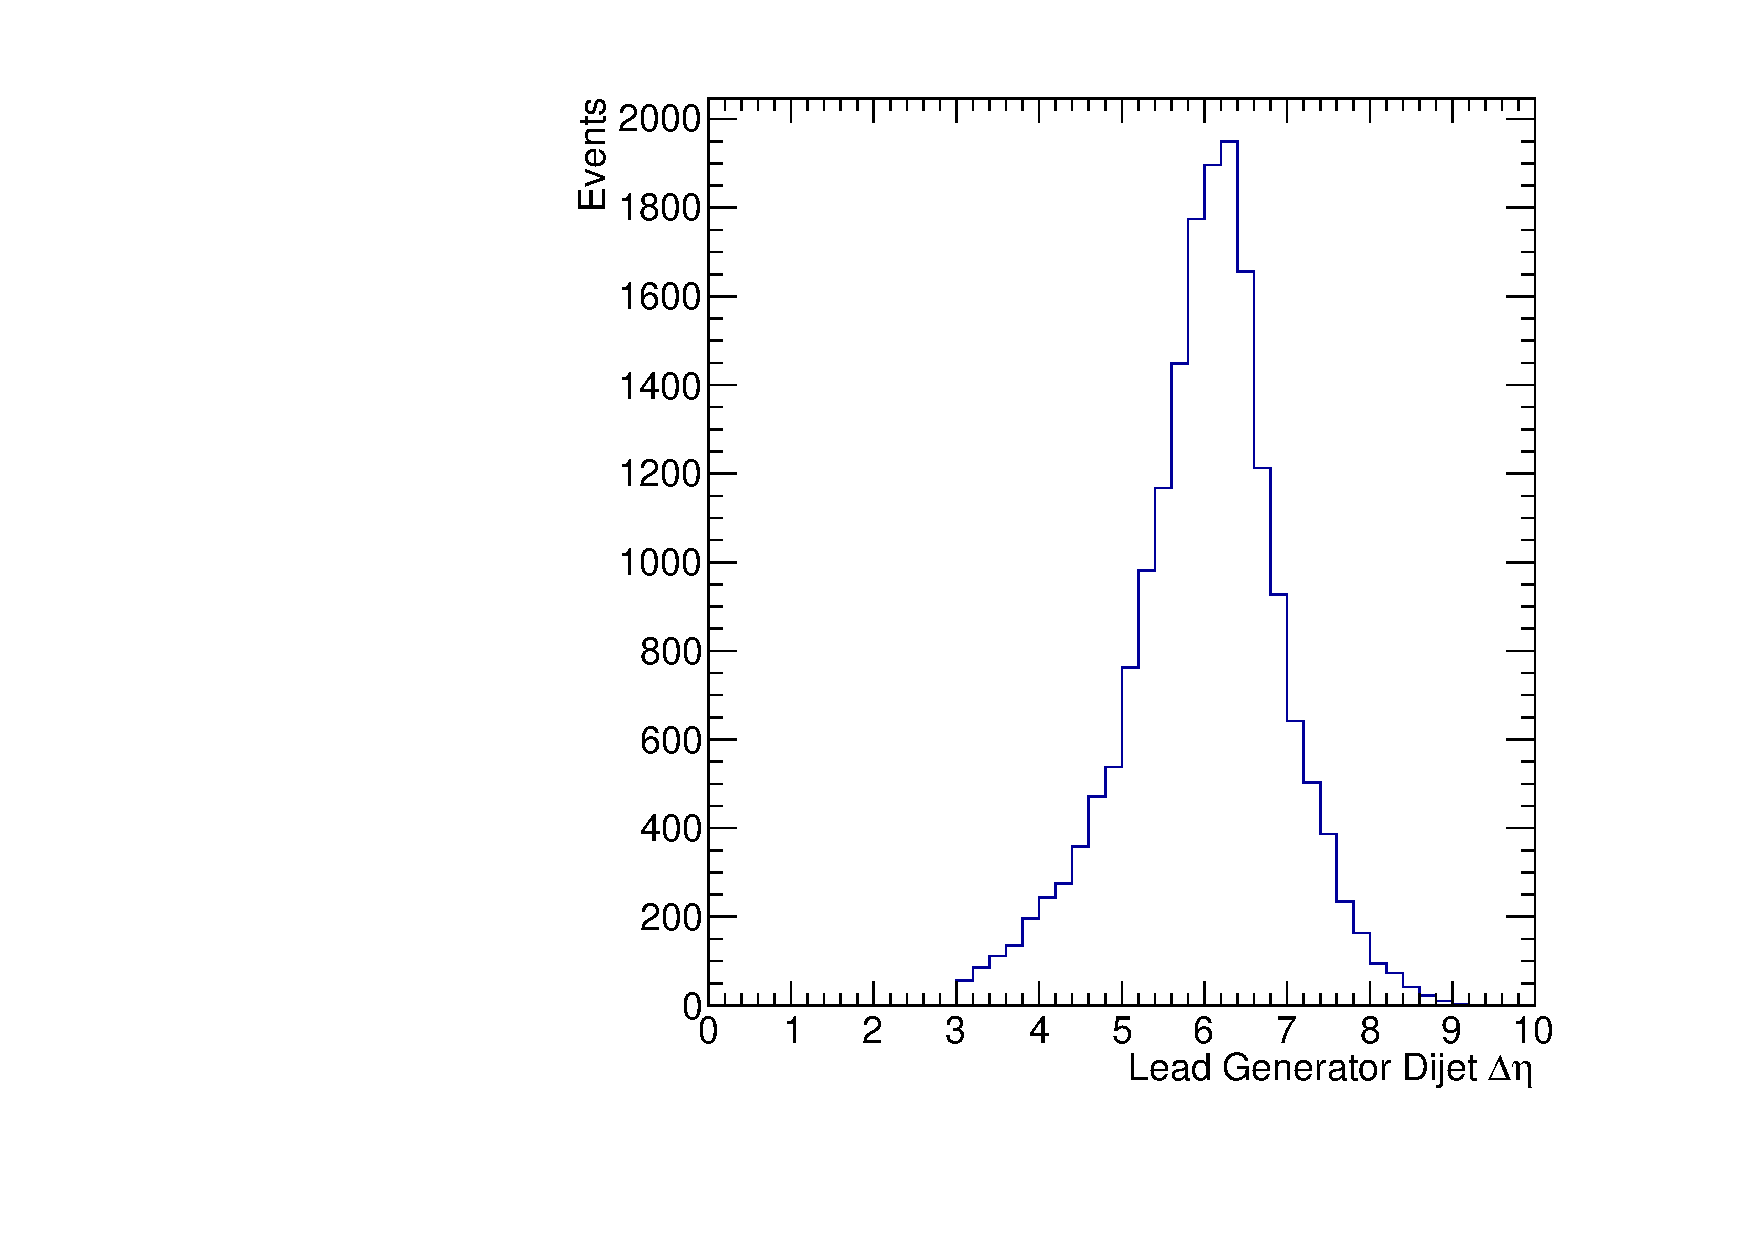
\includegraphics[width=0.40\linewidth]{Chapter07/QCDVBFSamples/GeneratorFilter/Pt40_Eta4p8_DEta3p0_Mjj1000/Images/LeadDijet_DEta.pdf}}\qquad
\subfloat[][]{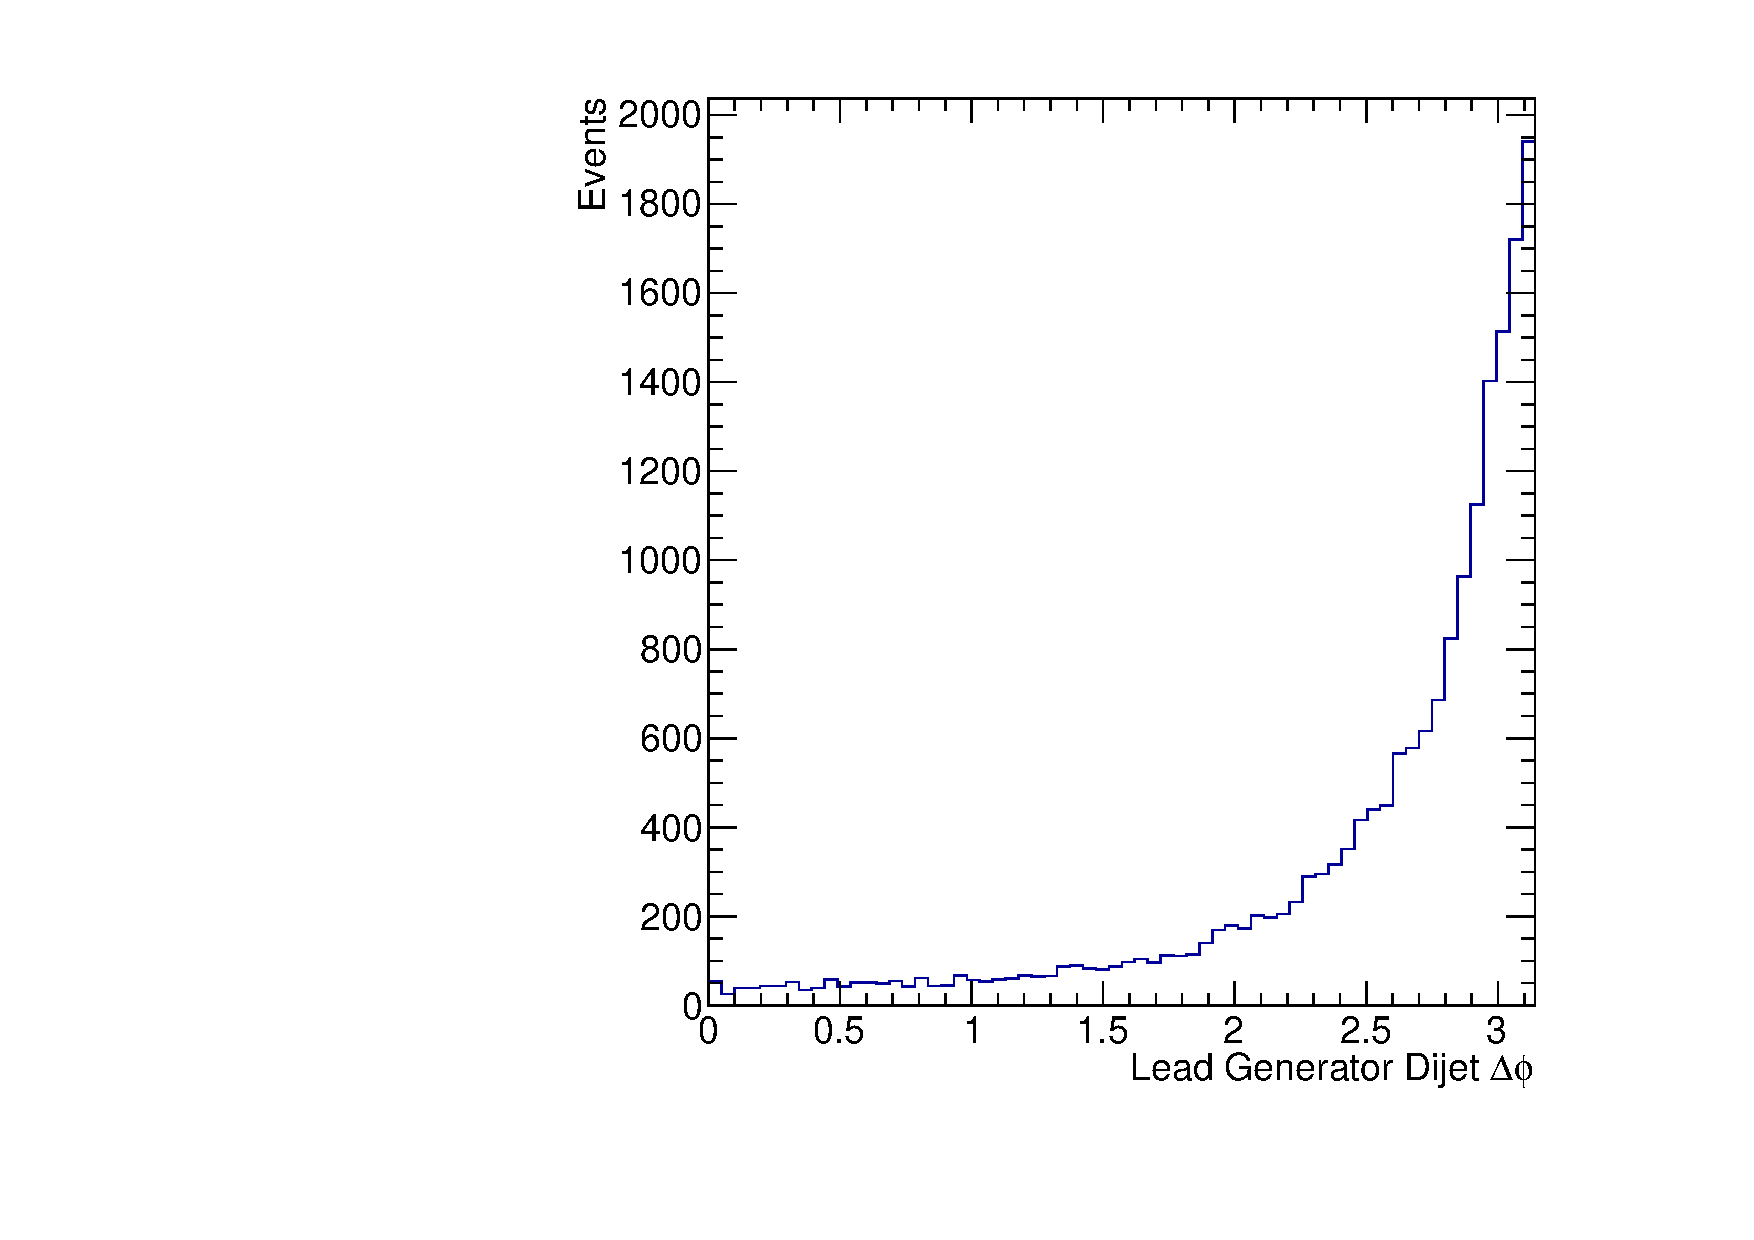
\includegraphics[width=0.40\linewidth]{Chapter07/QCDVBFSamples/GeneratorFilter/Pt40_Eta4p8_DEta3p0_Mjj1000/Images/LeadDijet_DPhi.pdf}}\\
\subfloat[][]{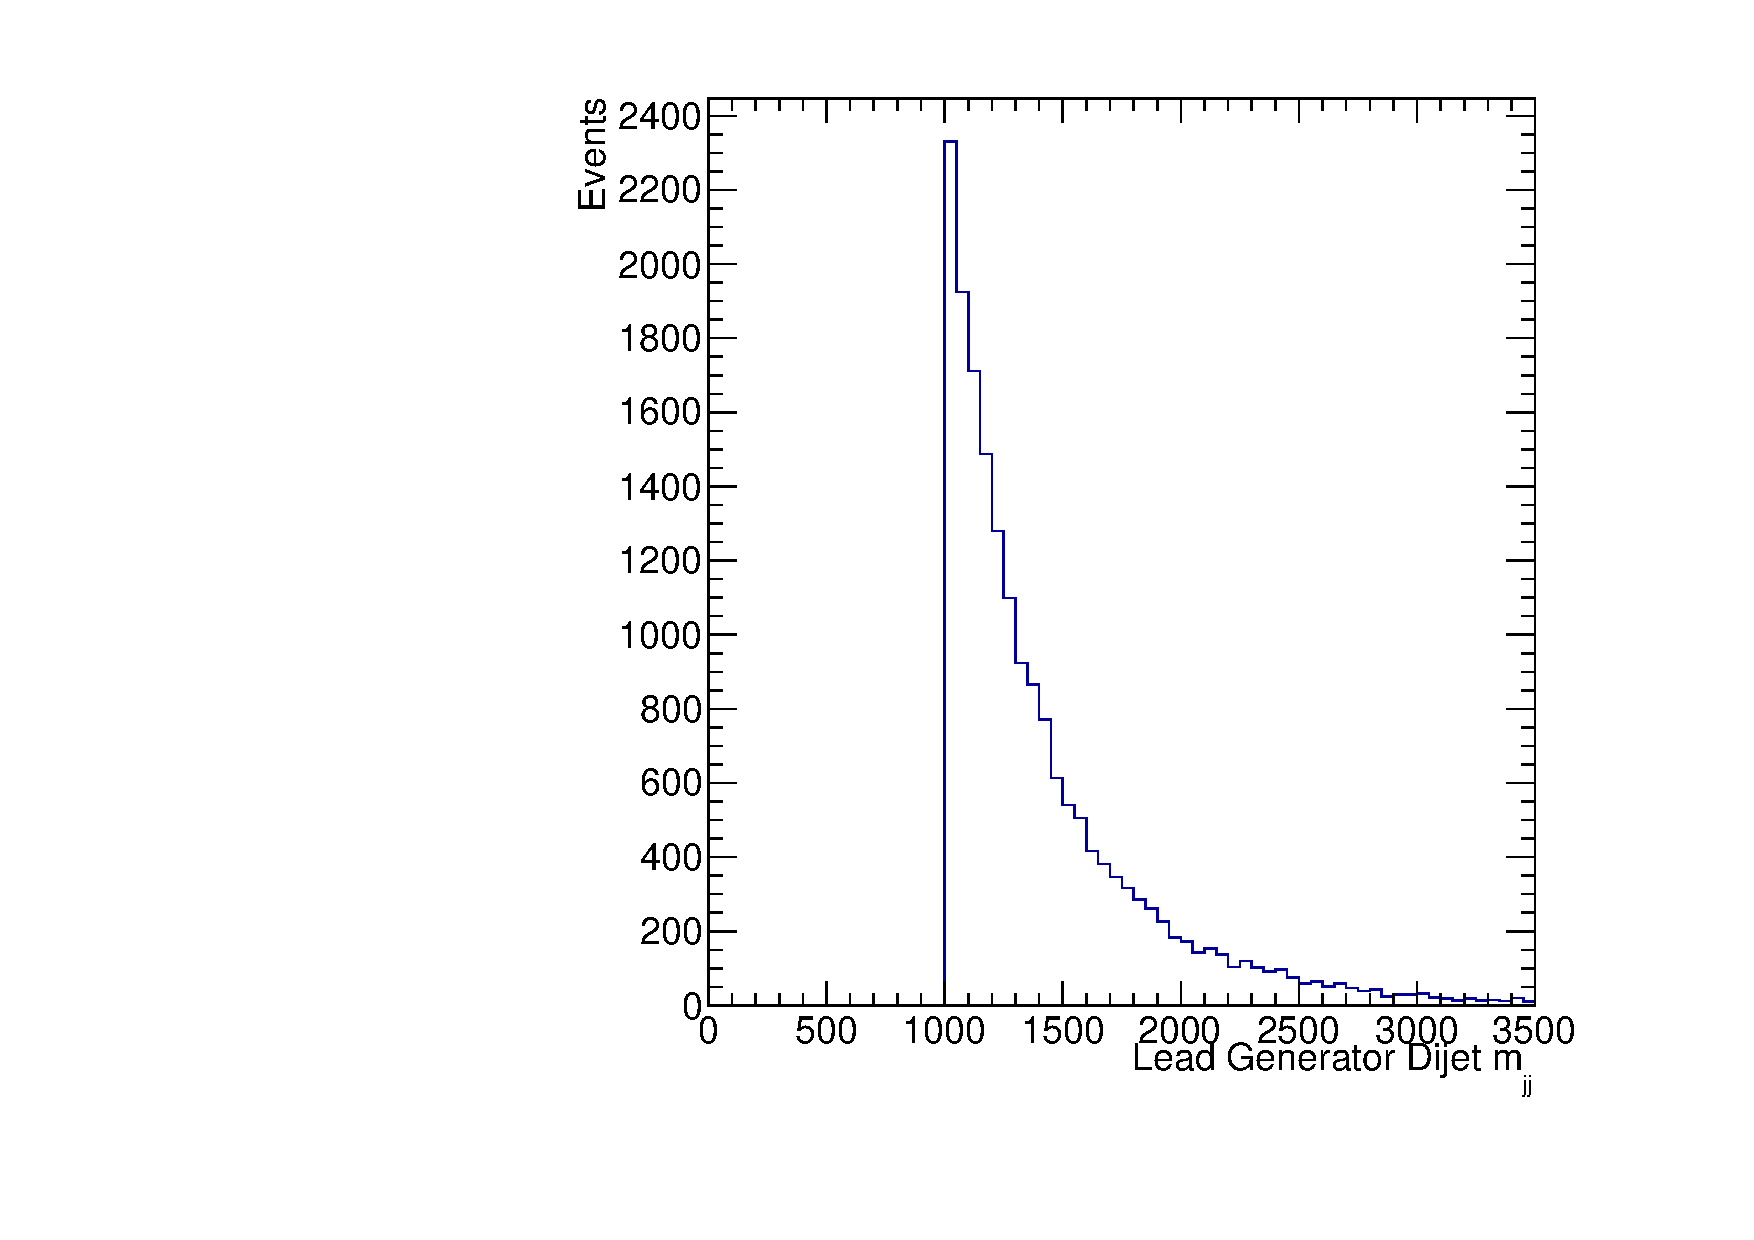
\includegraphics[width=0.40\linewidth]{Chapter07/QCDVBFSamples/GeneratorFilter/Pt40_Eta4p8_DEta3p0_Mjj1000/Images/LeadDijet_Mjj.pdf}}\\
\caption{Relevant distributions for the leading dijet passing a generator filter requiring at least one dijet with $\Delta\eta>3.0$ and $m_{jj}>1000\,\GeV$ where the jets have $\pt>40\,\GeV$ and $|\eta|<4.8$}
\label{FIGURE:RunIIPreparation_PassGeneratorFilterDistributions2}
\end{figure}

Sub-sample A will be produced by running over all the events produced up to the hadronization step. Its estimated filter efficiency is of $2.938 \times 10^{-1} \pm 4.67 \time 10^{-4}$ which would lead to a sample since of approximately 29 million events and corresponding to an equivalent luminosity of over $1.1\,\femto\barn^{-1}$.

Sub-sample B will result from running over only 10\% of the events available at the hadronization step. This filter has an efficiency of $1.125 \time 10^{-1} \pm 9.13 \time 10^{-4}$  and would lead to sample of about 14 million events, corresponding to an equivalent luminosity of over $110\,\pico\barn$. If additional computing resources would become available this sample could be expanded up to 100\% of the base sample to a total of 141 million events and equivalent luminosity over $1.1\,\femto\barn^{-1}$.

It is necessary to determine the overlap between this two sub-samples. From table \ref{TABLE:RunIIPreparation_PassFilterNJetsDphi} we can see that a significant amount of events on each sub-sample have additional jets, passing all required jet conditions. 

\begin{table}[!htp]
\centering
\begin{tabular}{|c||c|c|c|}
\hline
           & \multicolumn{3}{c|}{$\Delta\phi$ cut} \\
\hline
$N_{Jets}$ & no cut        & $<2.15$        & $\gtrsim 2.15$ \\
\hline\hline
 2         & 63.83 \pm 0.59 & 15.80 \pm 0.63 & 73.38 \pm 0.70 \\
 3         & 23.53 \pm 0.36 & 50.21 \pm 1.13 & 17.59 \pm 0.34 \\
 4         &  9.43 \pm 0.23 & 24.34 \pm 0.78 &  6.70 \pm 0.21 \\
 5         &  2.42 \pm 0.11 &  7.14 \pm 0.42 &  1.70 \pm 0.11 \\
+6         &  0.79 \pm 0.07 &  2.50 \pm 0.25 &  0.63 \pm 0.06 \\
\hline
\end{tabular}
\caption[Table showing the percentage of events for a given multiplicity of generator anti-$k_T$ jets with $R=0.4$ passing cuts $p_T>40\,\GeV$ and $|\eta|<4.8$. Only events with at least one such dijet with $\Delta\eta<3.0$ and $m_{jj}<1000\,\GeV$ are considered and results are presented according to a possible additional dijet $\Delta\phi$ cut.]
{Table showing the percentage of events for a given multiplicity of generator anti-$k_T$ jets with $R=0.4$ passing cuts $p_T>40\,\GeV$ and $|\eta|<4.8$. Only events with at least one such dijet with $\Delta\eta<3.0$ and $m_{jj}<1000\,\GeV$ are considered and results are presented according to a possible additional dijet $\Delta\phi$ cut.}
\label{TABLE:RunIIPreparation_PassFilterNJetsDphi}
\end{table}

% Information extracted to do this table:
%#######################################################
% Printing cuts: Pt40_Eta4p8_DEta3p0_Mjj1000
%#######################################################
% => Number Jets Passing pT and Eta cuts multiplicity (at least one combination passes all cuts):
% N_Jets= 0 entries=         0 fraction=0.000000 +/- 0.000000
% N_Jets= 1 entries=         0 fraction=0.000000 +/- 0.000000
% N_Jets= 2 entries=     11757 fraction=0.638274 +/- 0.005887
% N_Jets= 3 entries=      4335 fraction=0.235342 +/- 0.003574
% N_Jets= 4 entries=      1737 fraction=0.094300 +/- 0.002263
% N_Jets= 5 entries=       446 fraction=0.024213 +/- 0.001147
% N_Jets= 6 entries=       117 fraction=0.006352 +/- 0.000587
% N_Jets= 7 entries=        22 fraction=0.001194 +/- 0.000255
% N_Jets= 8 entries=         4 fraction=0.000217 +/- 0.000109
% N_Jets= 9 entries=         2 fraction=0.000109 +/- 0.000077
% N_Jets=10 entries=         0 fraction=0.000000 +/- 0.000000
%####################################################### 
% N_Jets=+6 entries=       145 fraction=0.007872 +/- 0.000654
%#######################################################
%
%
%######################################################
%Printing cuts: Pt40_Eta4p8_DEta3p0_Dphi2p15_Mjj1000
%######################################################
% => Number Jets Passing pT and Eta cuts multiplicity (at least one combination passes all cuts):
% N_Jets= 0 entries=         0 fraction=0.000000 +/- 0.000000
% N_Jets= 1 entries=         0 fraction=0.000000 +/- 0.000000
% N_Jets= 2 entries=       626 fraction=0.158041 +/- 0.006317
% N_Jets= 3 entries=      1989 fraction=0.502146 +/- 0.011259
% N_Jets= 4 entries=       964 fraction=0.243373 +/- 0.007839
% N_Jets= 5 entries=       283 fraction=0.071447 +/- 0.004247
% N_Jets= 6 entries=        81 fraction=0.020449 +/- 0.002272
% N_Jets= 7 entries=        15 fraction=0.003787 +/- 0.000978
% N_Jets= 8 entries=         2 fraction=0.000505 +/- 0.000357
% N_Jets= 9 entries=         1 fraction=0.000252 +/- 0.000252
% N_Jets=10 entries=         0 fraction=0.000000 +/- 0.000000
%####################################################### 
% N_Jets=+6 entries=        99 fraction=0.024994 +/- 0.002512
%####################################################### 
%
%
%#######################################################
%Printing cuts: Pt40_Eta4p8_DEta3p0_MinDphi2p15_Mjj1000
%####################################################### 
% => Number Jets Passing pT and Eta cuts multiplicity (at least one combination passes all cuts):
% N_Jets= 0 entries=         0 fraction=0.000000 +/- 0.000000
% N_Jets= 1 entries=         0 fraction=0.000000 +/- 0.000000
% N_Jets= 2 entries=     11131 fraction=0.733799 +/- 0.006955
% N_Jets= 3 entries=      2668 fraction=0.175885 +/- 0.003405
% N_Jets= 4 entries=      1017 fraction=0.067045 +/- 0.002102
% N_Jets= 5 entries=       258 fraction=0.017008 +/- 0.001059
% N_Jets= 6 entries=        75 fraction=0.004944 +/- 0.000571
% N_Jets= 7 entries=        15 fraction=0.000989 +/- 0.000255
% N_Jets= 8 entries=         3 fraction=0.000198 +/- 0.000114
% N_Jets= 9 entries=         2 fraction=0.000132 +/- 0.000093
% N_Jets=10 entries=         0 fraction=0.000000 +/- 0.000000
%#######################################################
% N_Jets=+6 entries=        95 fraction=0.006263 +/- 0.000643
%#######################################################


This additional jets lead to additional combinations that may pass the criteria of the opposite sub-sample. As it can be seen in table \ref{TABLE:RunIIPreparation_PassFilterNDijetsDphi} in as much as 5\% of the events in the $\Delta\phi<=2.15$ sub-sample there is a second combination of two jets that would pass the criteria to be in that sub-sample.

\begin{table}[!htp]
\centering
\begin{tabular}{|c|c|c|c|}
\hline
           & \multicolumn{3}{c|}{$\Delta\phi$ cut} \\
\hline
$N_{Jets}$ & no cut        & $<2.15$        & $\gtrsim 2.15$ \\
\hline\hline
 1         & 93.53 \pm 0.71 & 94.29 \pm 1.54 & 97.51 \pm 0.80 \\
 2         &  5.84 \pm 0.18 &  5.35 \pm 0.37 &  2.39 \pm 0.13 \\
 3         &  0.44 \pm 0.05 &  0.30 \pm 0.09 &  0.07 \pm 0.02 \\
+4         &  0.19 \pm 0.03 &  0.05 \pm 0.04 &  0.03 \pm 0.01 \\
\hline
\end{tabular}
\caption{Table showing the percentage of generator AK4 dijets passing cuts $p_T^{jet}>40\,\GeV$, $|\eta|^{jet}<4.8$, $\Delta\eta<3.0$ and $m_{jj}<1000\,\GeV$ and according to an additional dijet $\Delta\phi$ cut.}
\end{table}

% #######################################################
% Printing cuts: Pt40_Eta4p8_DEta3p0_Mjj1000
% #######################################################
% => Dijets passing all cuts multiplicity:
% N_Dijets= 0 entries=         0 fraction=0.000000 +/- 0.000000
% N_Dijets= 1 entries=     17228 fraction=0.935288 +/- 0.007126
% N_Dijets= 2 entries=      1076 fraction=0.058415 +/- 0.001781
% N_Dijets= 3 entries=        81 fraction=0.004397 +/- 0.000489
% N_Dijets= 4 entries=        31 fraction=0.001683 +/- 0.000302
% N_Dijets= 5 entries=         2 fraction=0.000109 +/- 0.000077
% N_Dijets= 6 entries=         2 fraction=0.000109 +/- 0.000077
% N_Dijets= 7 entries=         0 fraction=0.000000 +/- 0.000000
% N_Dijets= 8 entries=         0 fraction=0.000000 +/- 0.000000
% N_Dijets= 9 entries=         0 fraction=0.000000 +/- 0.000000
% N_Dijets=10 entries=         0 fraction=0.000000 +/- 0.000000
% ####################################################### 
% N_Dijets=+4 entries=        35 fraction=0.001900 +/- 0.000321
% #######################################################
%
% 
% #######################################################
% Printing cuts: Pt40_Eta4p8_DEta3p0_Dphi2p15_Mjj1000
% #######################################################
% => Dijets passing all cuts multiplicity:
% N_Dijets= 0 entries=         0 fraction=0.000000 +/- 0.000000
% N_Dijets= 1 entries=      3735 fraction=0.942944 +/- 0.015429
% N_Dijets= 2 entries=       212 fraction=0.053522 +/- 0.003676
% N_Dijets= 3 entries=        12 fraction=0.003030 +/- 0.000875
% N_Dijets= 4 entries=         2 fraction=0.000505 +/- 0.000357
% N_Dijets= 5 entries=         0 fraction=0.000000 +/- 0.000000
% N_Dijets= 6 entries=         0 fraction=0.000000 +/- 0.000000
% N_Dijets= 7 entries=         0 fraction=0.000000 +/- 0.000000
% N_Dijets= 8 entries=         0 fraction=0.000000 +/- 0.000000
% N_Dijets= 9 entries=         0 fraction=0.000000 +/- 0.000000
% N_Dijets=10 entries=         0 fraction=0.000000 +/- 0.000000
% ####################################################### 
%
% #######################################################
% 
% 
% #######################################################
% Printing cuts: Pt40_Eta4p8_DEta3p0_MinDphi2p15_Mjj1000
% #######################################################
% => Dijets passing all cuts multiplicity:
% N_Dijets= 0 entries=         0 fraction=0.000000 +/- 0.000000
% N_Dijets= 1 entries=     14791 fraction=0.975081 +/- 0.008018
% N_Dijets= 2 entries=       363 fraction=0.023930 +/- 0.001256
% N_Dijets= 3 entries=        11 fraction=0.000725 +/- 0.000219
% N_Dijets= 4 entries=         4 fraction=0.000264 +/- 0.000132
% N_Dijets= 5 entries=         0 fraction=0.000000 +/- 0.000000
% N_Dijets= 6 entries=         0 fraction=0.000000 +/- 0.000000
% N_Dijets= 7 entries=         0 fraction=0.000000 +/- 0.000000
% N_Dijets= 8 entries=         0 fraction=0.000000 +/- 0.000000
% N_Dijets= 9 entries=         0 fraction=0.000000 +/- 0.000000
% N_Dijets=10 entries=         0 fraction=0.000000 +/- 0.000000
% ####################################################### 
%
% #######################################################


The overlap between the two sub-samples has been determined to be $3.95\% \pm 0.14\%$ of the events passing the initial selection. Since this number is relevant, and to to avoid event double counting, events with combinations that would pass both sub-sample definitions should be vetoed in one of the samples.

%%%%%%%%%%%%%%%%%%%%%%%%%%%%%%%%%%%%%%%%%%%%%%%%%%%%%%%%%%%%%%%%%%%%%%%%%%%%%%%%%%%%%%%
%%% SUBSECTION
%%%%%%%%%%%%%%%%%%%%%%%%%%%%%%%%%%%%%%%%%%%%%%%%%%%%%%%%%%%%%%%%%%%%%%%%%%%%%%%%%%%%%%%
\subsection{Migration study}
\label{SUBSECTION:RunIIPreparation_MigrationStudy}

%Status: DONE

On concern when making cuts at steps below event reconstruction is the possibility of cutting events that may pass analysis event selections. This migration of events needs to be taken into account while defining the cuts at parton and generator levels. If we take the relevant variables of signal region selection used during the 2012-13 parked data analysis, we selected a dijet with   $\Delta\eta>3.6$ and dijet $m_{jj}>1200\,\GeV$ where the lead jet $\pt > 50\,\GeV$ and sub-lead jet $\pt > 45\,\GeV$ and both have $|\eta|<4.7$ (condition to guarantee the used AK5 jets are fully contained in the detector). It is unlikely that the Run II offline selection would be able to cut below jet $\pt > 50\,\GeV$.

In order to study migration a second \gls{MC} sample with lower parton cuts was generated. We also used MadGraph as an event generator with all the same parameters with the only difference being the dijet cuts. We now select events with at least a pair of outgoing partons with invariant mass of $600\,\GeV$, where both parton are inside the detector volume with $|\eta|<5.0$ and have more than $p_{T}>10\,\GeV$. Hadronization was then performed with the same procedure described in the previous section.

In order to compare generator jets to the partons that created them we need to match them. For each parton we select all generator jet which are located at $\Delta R < 0.4$ and from those we select the generator jet with less difference of \pt to our parton. This procedure attempts to account for situation where more than one jet is within the matching distance but the best match in \pt is not the closest one in $\Delta R$. Using this procedure we can find a match for the di-parton passing the imposed cuts for 73.24\% of the events and we also find that the matched generator jet is not the closest one in $\Delta R$ for 3.45\% of the partons. A table of the matching efficiency for discriminated by physics process can be found in table \ref{TABLE:RunIIPreparation_PartonGenJetMatchingEfficiency}. 

\begin{table}[!htp]
\centering

\begin{tabular}{|c||c|c|c||c|}
\hline
            &          \multicolumn{4}{c|}{Process} \\
\hline
$n_{match}$ &      jj &    jjj  &    jjjj &   Total \\
\hline\hline 
          0 & 22.04\% \pm 0.22\%  &  2.18\% \pm  0.09\% &  0.14\% \pm  0.03\% & 11.62\% \pm 0.11\% \\
          1 & 38.60\% \pm 0.30\%  & 17.82\% \pm  0.25\% &  3.02\% \pm  0.13\% & 25.27\% \pm 0.17\% \\
          2 & 39.35\% \pm 0.30\%  & 42.35\% \pm  0.39\% & 16.91\% \pm  0.32\% & 35.99\% \pm 0.20\% \\
          3 &                     & 37.65\% \pm  0.37\% & 41.88\% \pm  0.50\% & 19.83\% \pm 0.15\% \\
          4 &                     &                     & 38.05\% \pm  0.47\% &  7.29\% \pm 0.09\% \\
\hline
\end{tabular}
\caption{Table showing the percentage of partons successfully matched to a generator AK4 jets. Numbers obtained for a total of 88282 events over all 3 possible hard scattering processes and for events with at least on di-parton with $m_{jj}>600\,GeV$ where each parton has $\pt < 10\,\GeV$ and $|\eta|<5.0$}
\label{TABLE:RunIIPreparation_PartonGenJetMatchingEfficiency}
\end{table}               

% => Parton to GenJet matching results:                                                                                                                                       
% all partons entries 88282                                                                                                                                                   
% Matched #0 partons:  10257 percentage: 11.62 +/-  0.11                                                                                                                      
% Matched #1 partons:  22308 percentage: 25.27 +/-  0.17                                                                                                                      
% Matched #2 partons:  31771 percentage: 35.99 +/-  0.20                                                                                                                      
% Matched #3 partons:  17506 percentage: 19.83 +/-  0.15                                                                                                                      
% Matched #4 partons:   6440 percentage:  7.29 +/-  0.09                                                                                                                      
% 
% jj partons entries 43689                                                                                                                                                    
% Matched #0 partons:   9631 percentage: 22.04 +/-  0.22                                                                                                                      
% Matched #1 partons:  16866 percentage: 38.60 +/-  0.30                                                                                                                      
% Matched #2 partons:  17192 percentage: 39.35 +/-  0.30                                                                                                                      
% 
% jjj partons entries 27667                                                                                                                                                   
% Matched #0 partons:    603 percentage:  2.18 +/-  0.09                                                                                                                      
% Matched #1 partons:   4930 percentage: 17.82 +/-  0.25                                                                                                                      
% Matched #2 partons:  11716 percentage: 42.35 +/-  0.39                                                                                                                      
% Matched #3 partons:  10418 percentage: 37.65 +/-  0.37                                                                                                                      
% 
% jjjj partons entries 16926                                                                                                                                                  
% Matched #0 partons:     23 percentage:  0.14 +/-  0.03                                                                                                                      
% Matched #1 partons:    512 percentage:  3.02 +/-  0.13                                                                                                                      
% Matched #2 partons:   2863 percentage: 16.91 +/-  0.32                                                                                                                      
% Matched #3 partons:   7088 percentage: 41.88 +/-  0.50                                                                                                                      
% Matched #4 partons:   6440 percentage: 38.05 +/-  0.47 




Since we are simulating partons with fairly low \pt, two jets with $\pt > 10\,\GeV$ and up to two more with no restriction on energy. It is not a surprise that in significant amount of events we cannot match all partons to generator jets. This is due to the spread of energy over a larger area then the jet algorithm can cluster and due to the default AK4 minimum \pt necessary to form a jet of $3\,\GeV$. A set of plots of the of the relevant variable are plotted in figure \ref{FIGURE:RunIIPreparation_VariablesPartonVsGenJet}. Here we take the selected di-parton and plot each variable against the matched dijet.


\begin{figure}[!htp]%
\centering
\subfloat[][]{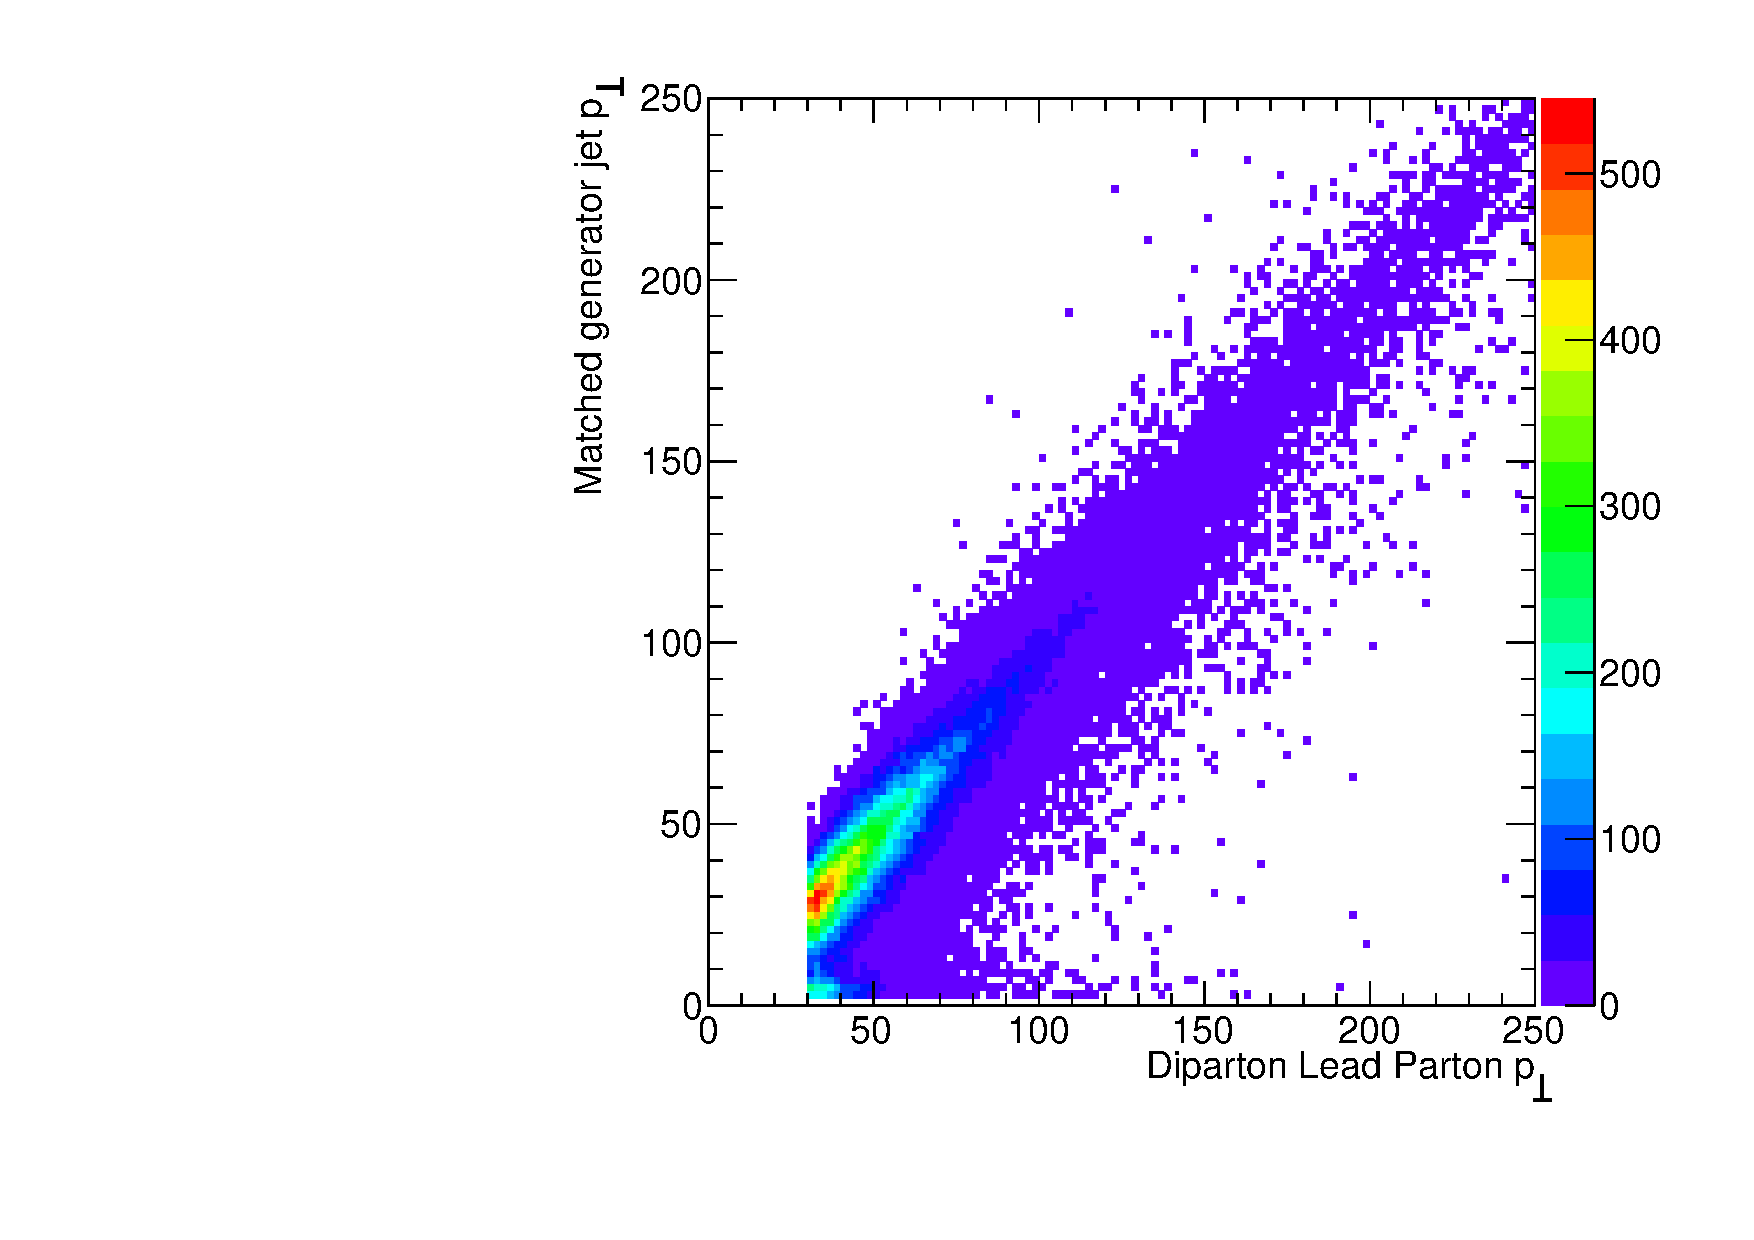
\includegraphics[width=0.40\linewidth]{Chapter07/QCDVBFSamples/Migrations/Images/SelDiParton_MatchedGenJet_Parton1_Pt.pdf}}\qquad
\subfloat[][]{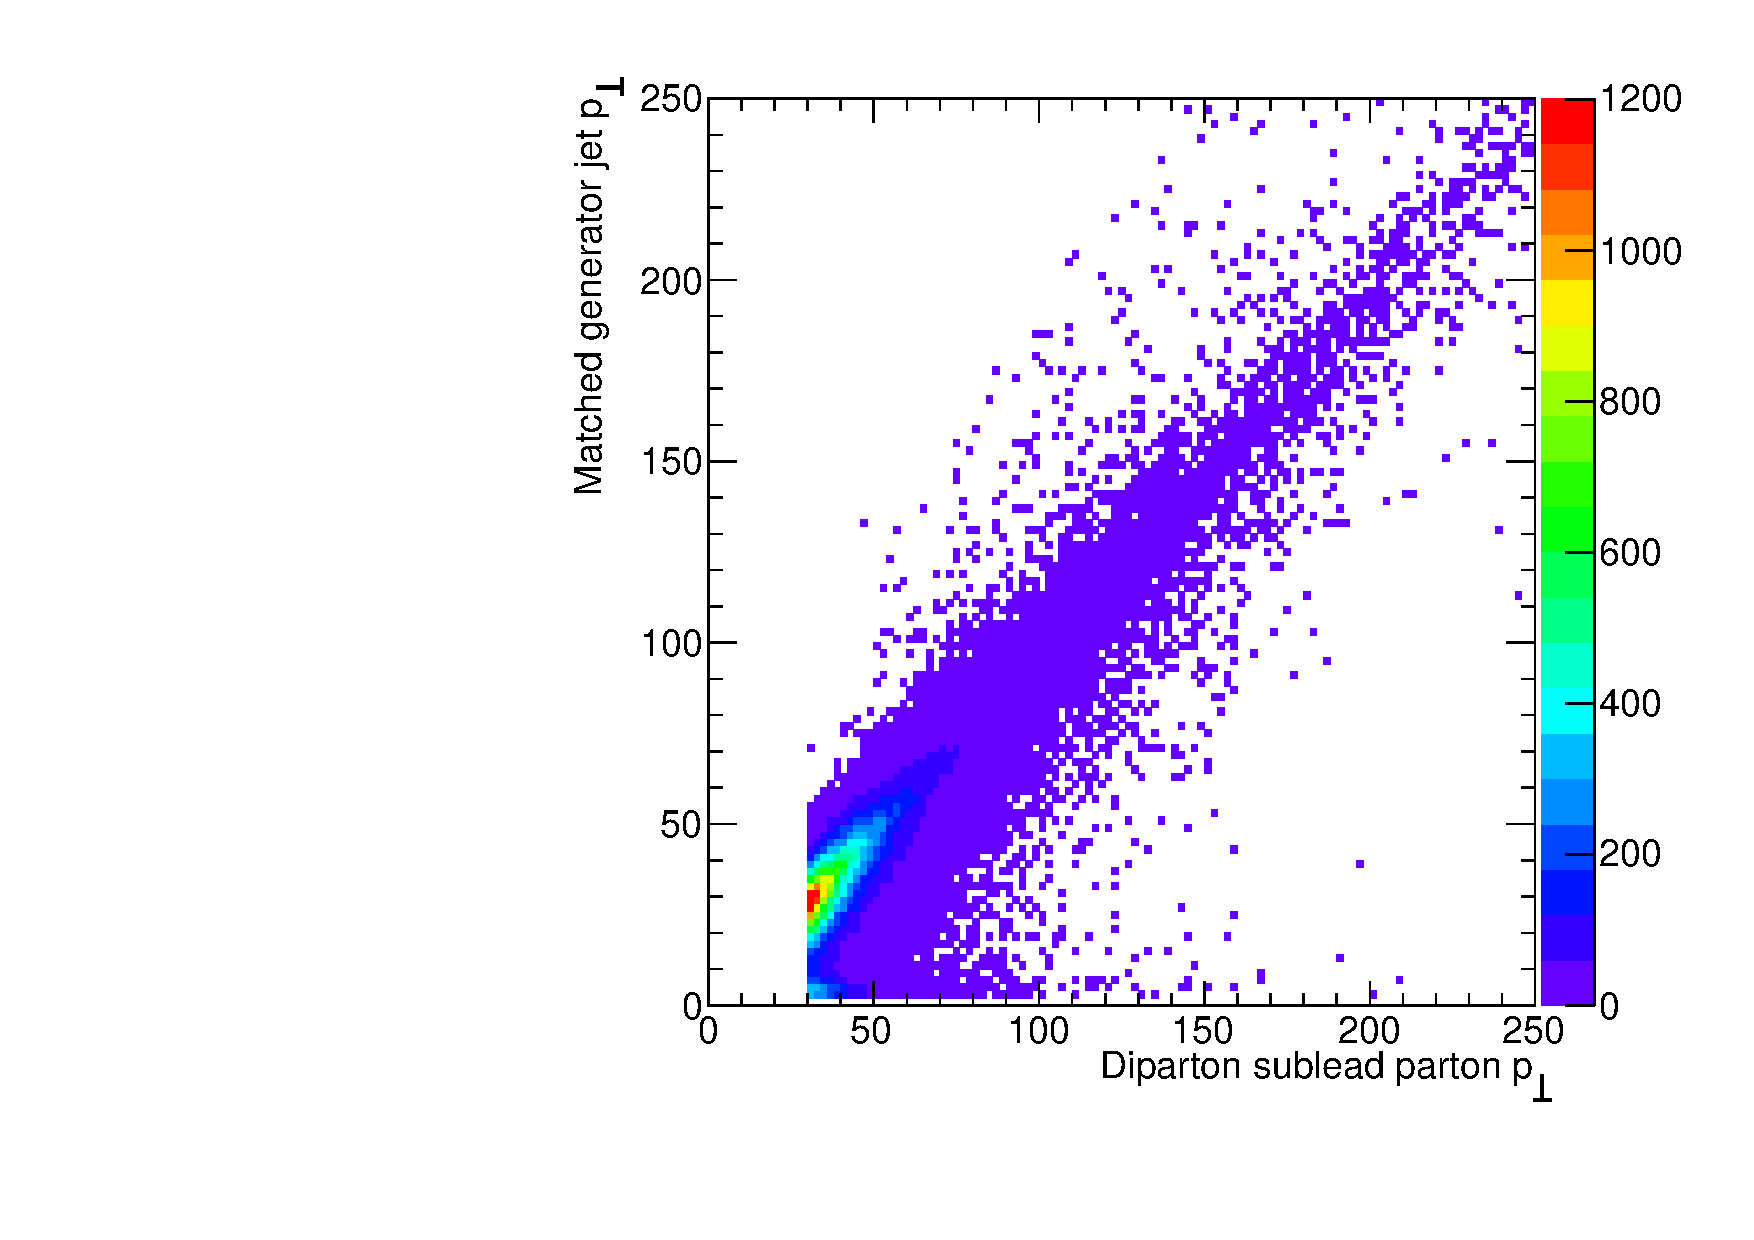
\includegraphics[width=0.40\linewidth]{Chapter07/QCDVBFSamples/Migrations/Images/SelDiParton_MatchedGenJet_Parton2_Pt.pdf}}\\
\subfloat[][]{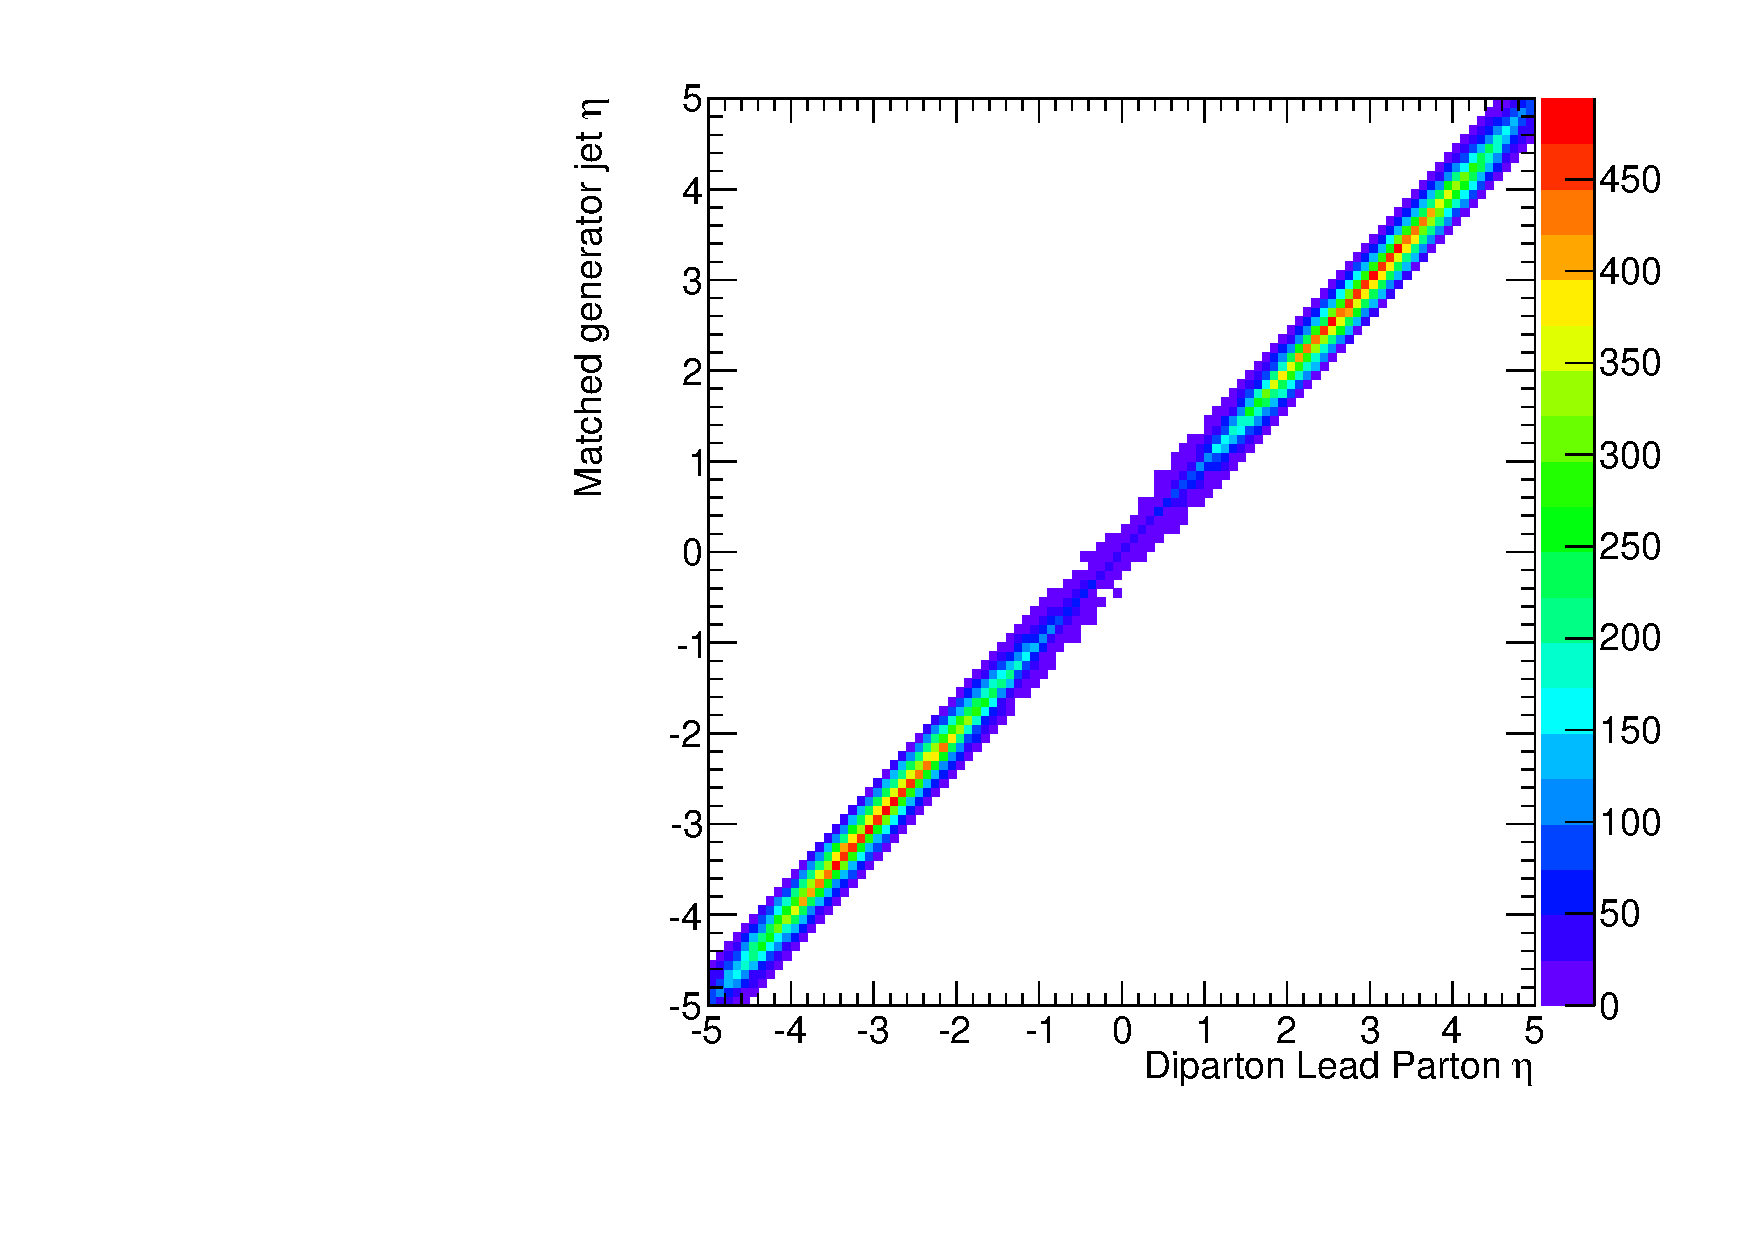
\includegraphics[width=0.40\linewidth]{Chapter07/QCDVBFSamples/Migrations/Images/SelDiParton_MatchedGenJet_Parton1_Eta.pdf}}\qquad
\subfloat[][]{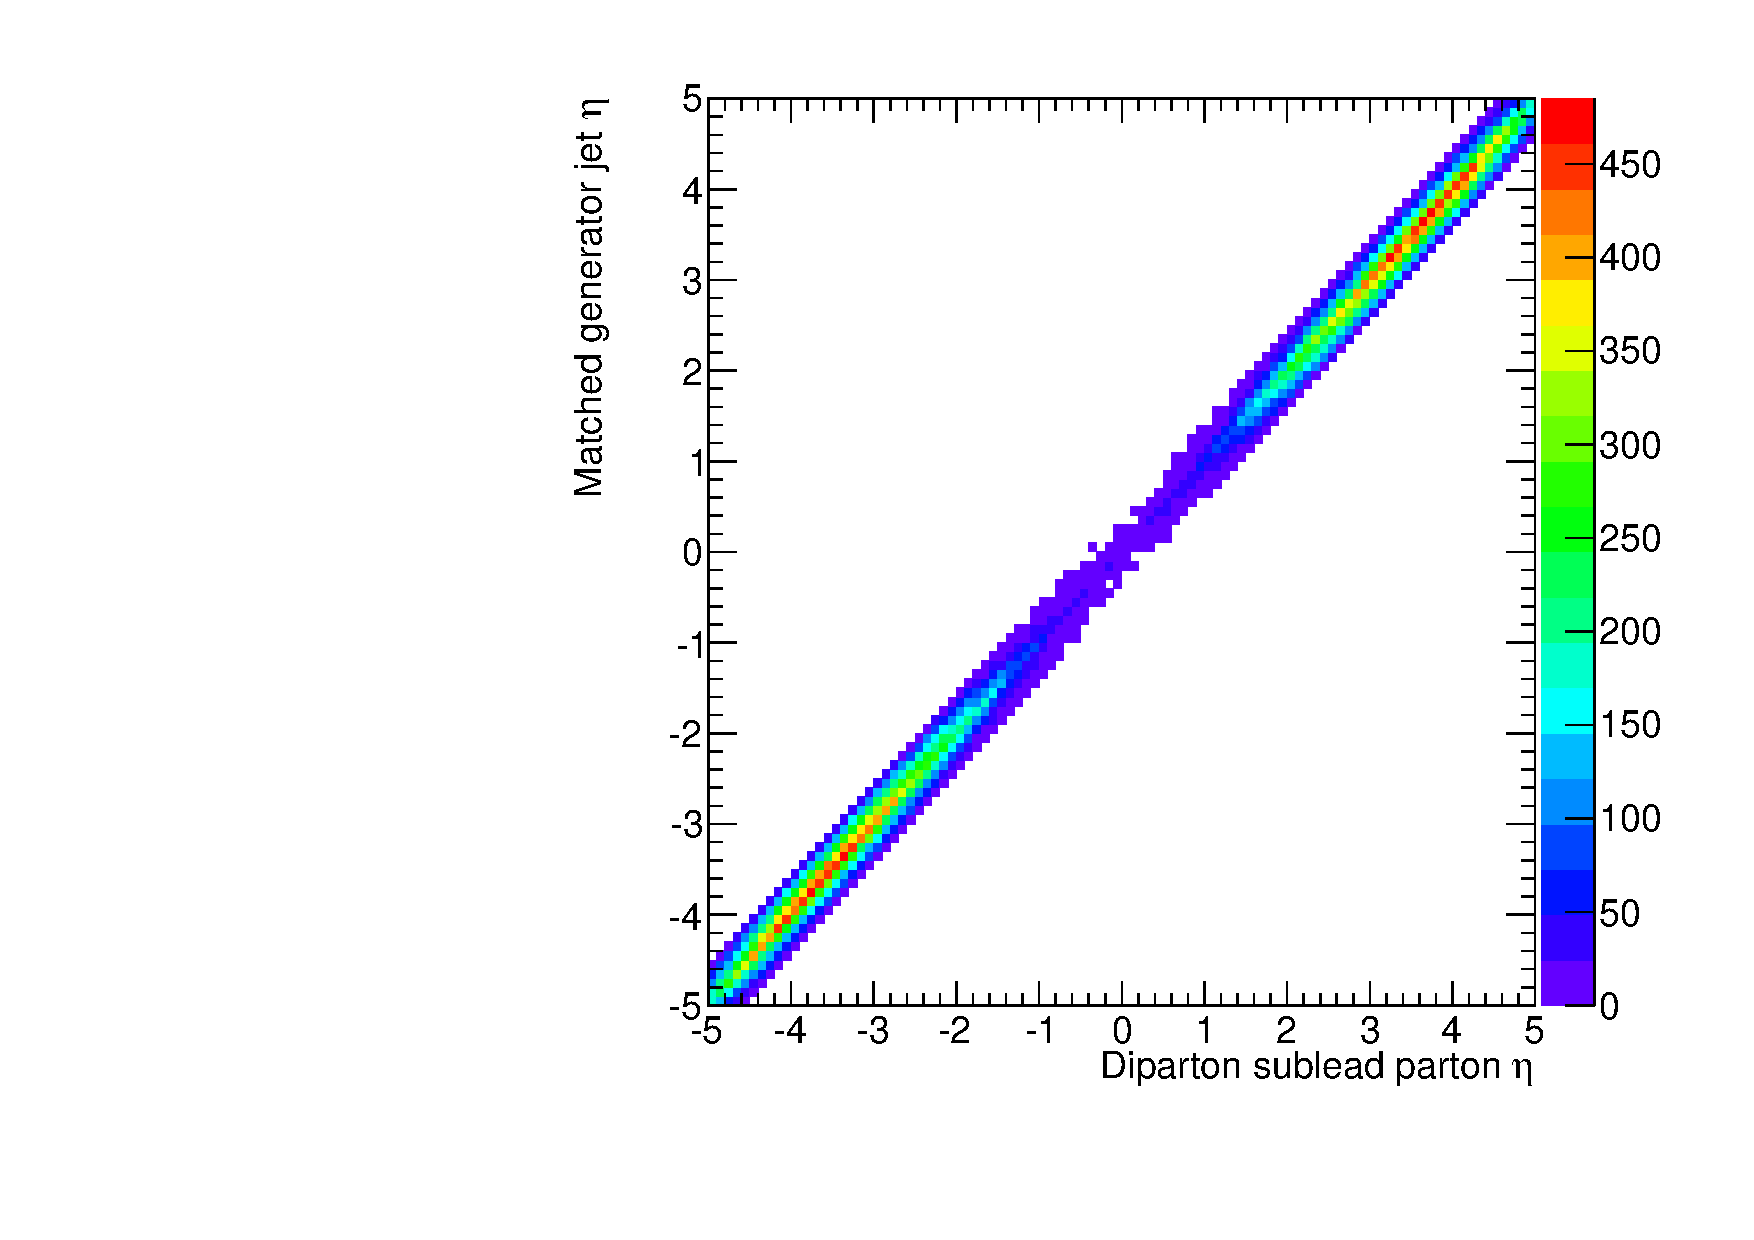
\includegraphics[width=0.40\linewidth]{Chapter07/QCDVBFSamples/Migrations/Images/SelDiParton_MatchedGenJet_Parton2_Eta.pdf}}\\
\subfloat[][]{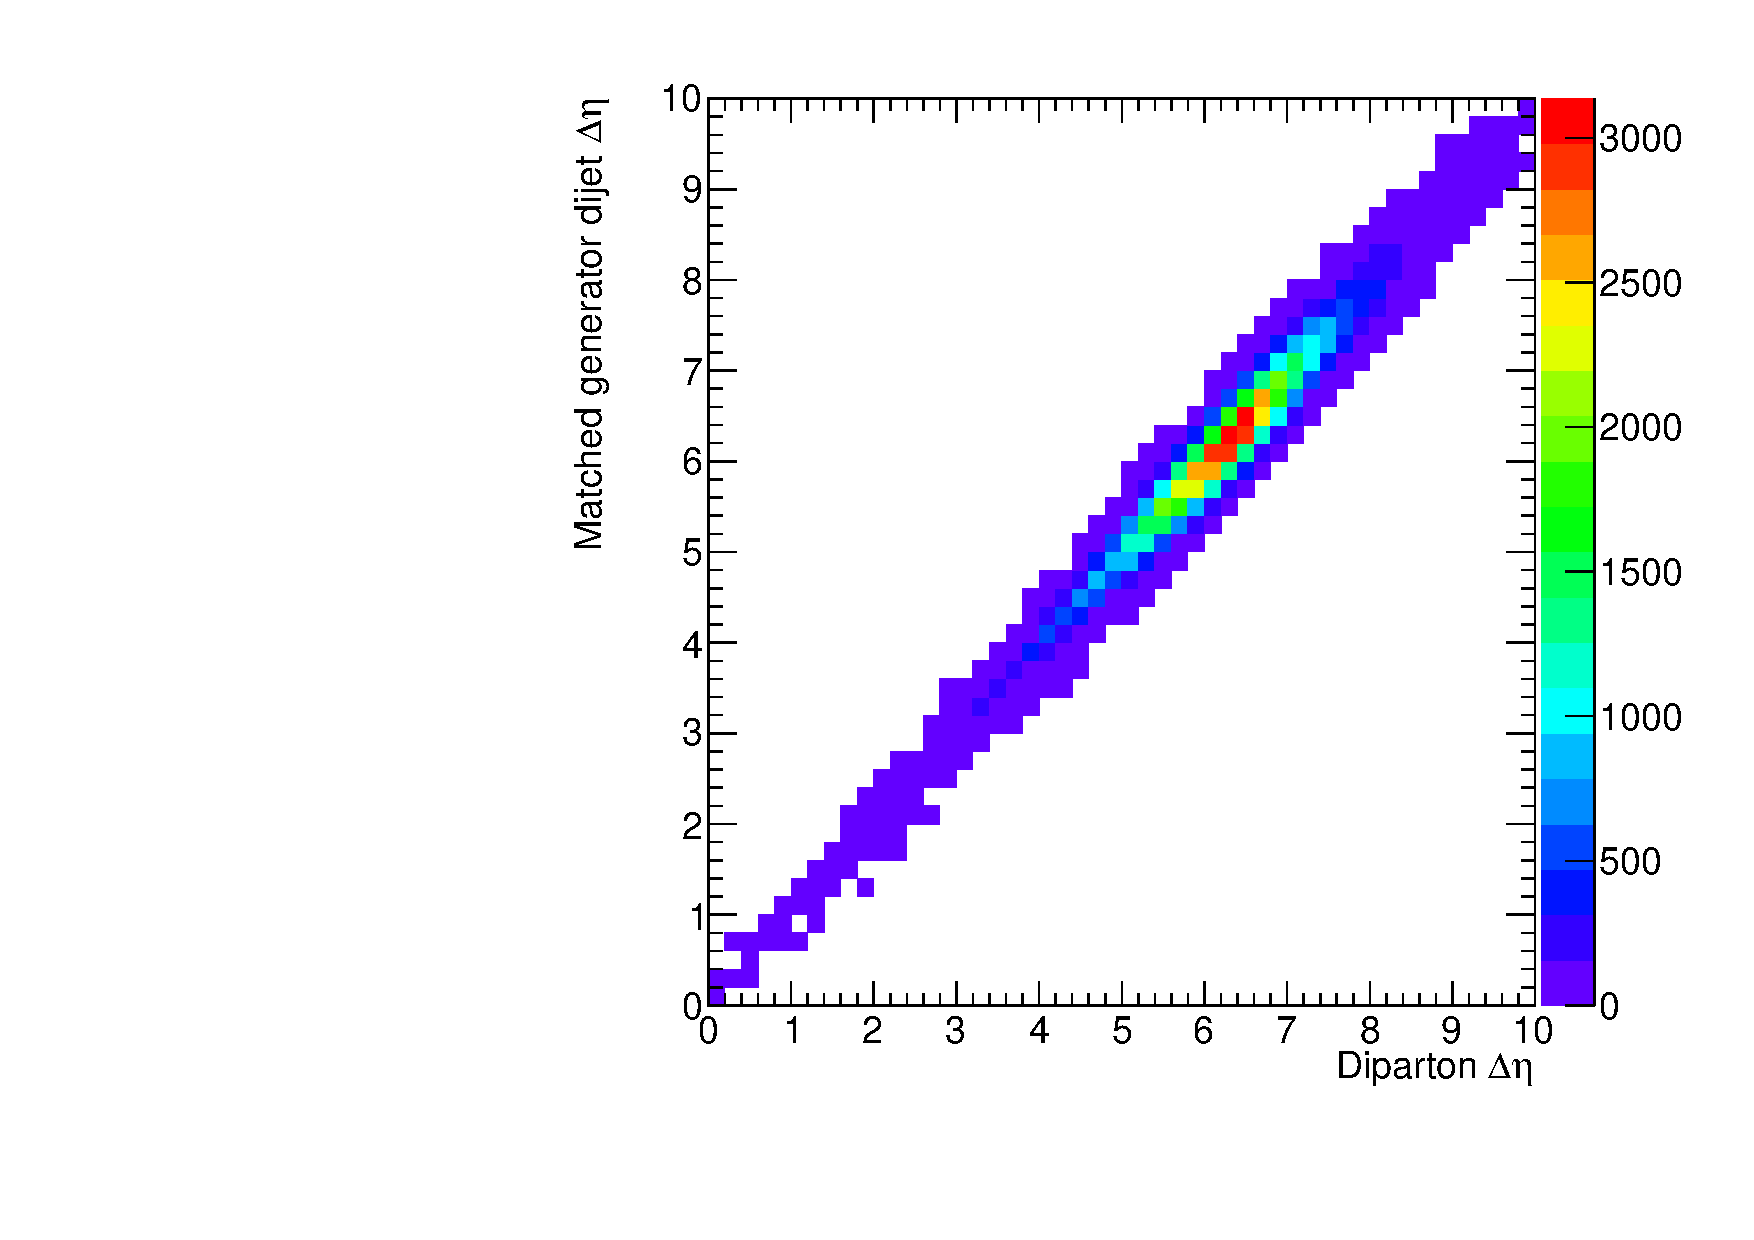
\includegraphics[width=0.40\linewidth]{Chapter07/QCDVBFSamples/Migrations/Images/SelDiParton_MatchedGenJet_DEta.pdf}}\qquad
\subfloat[][]{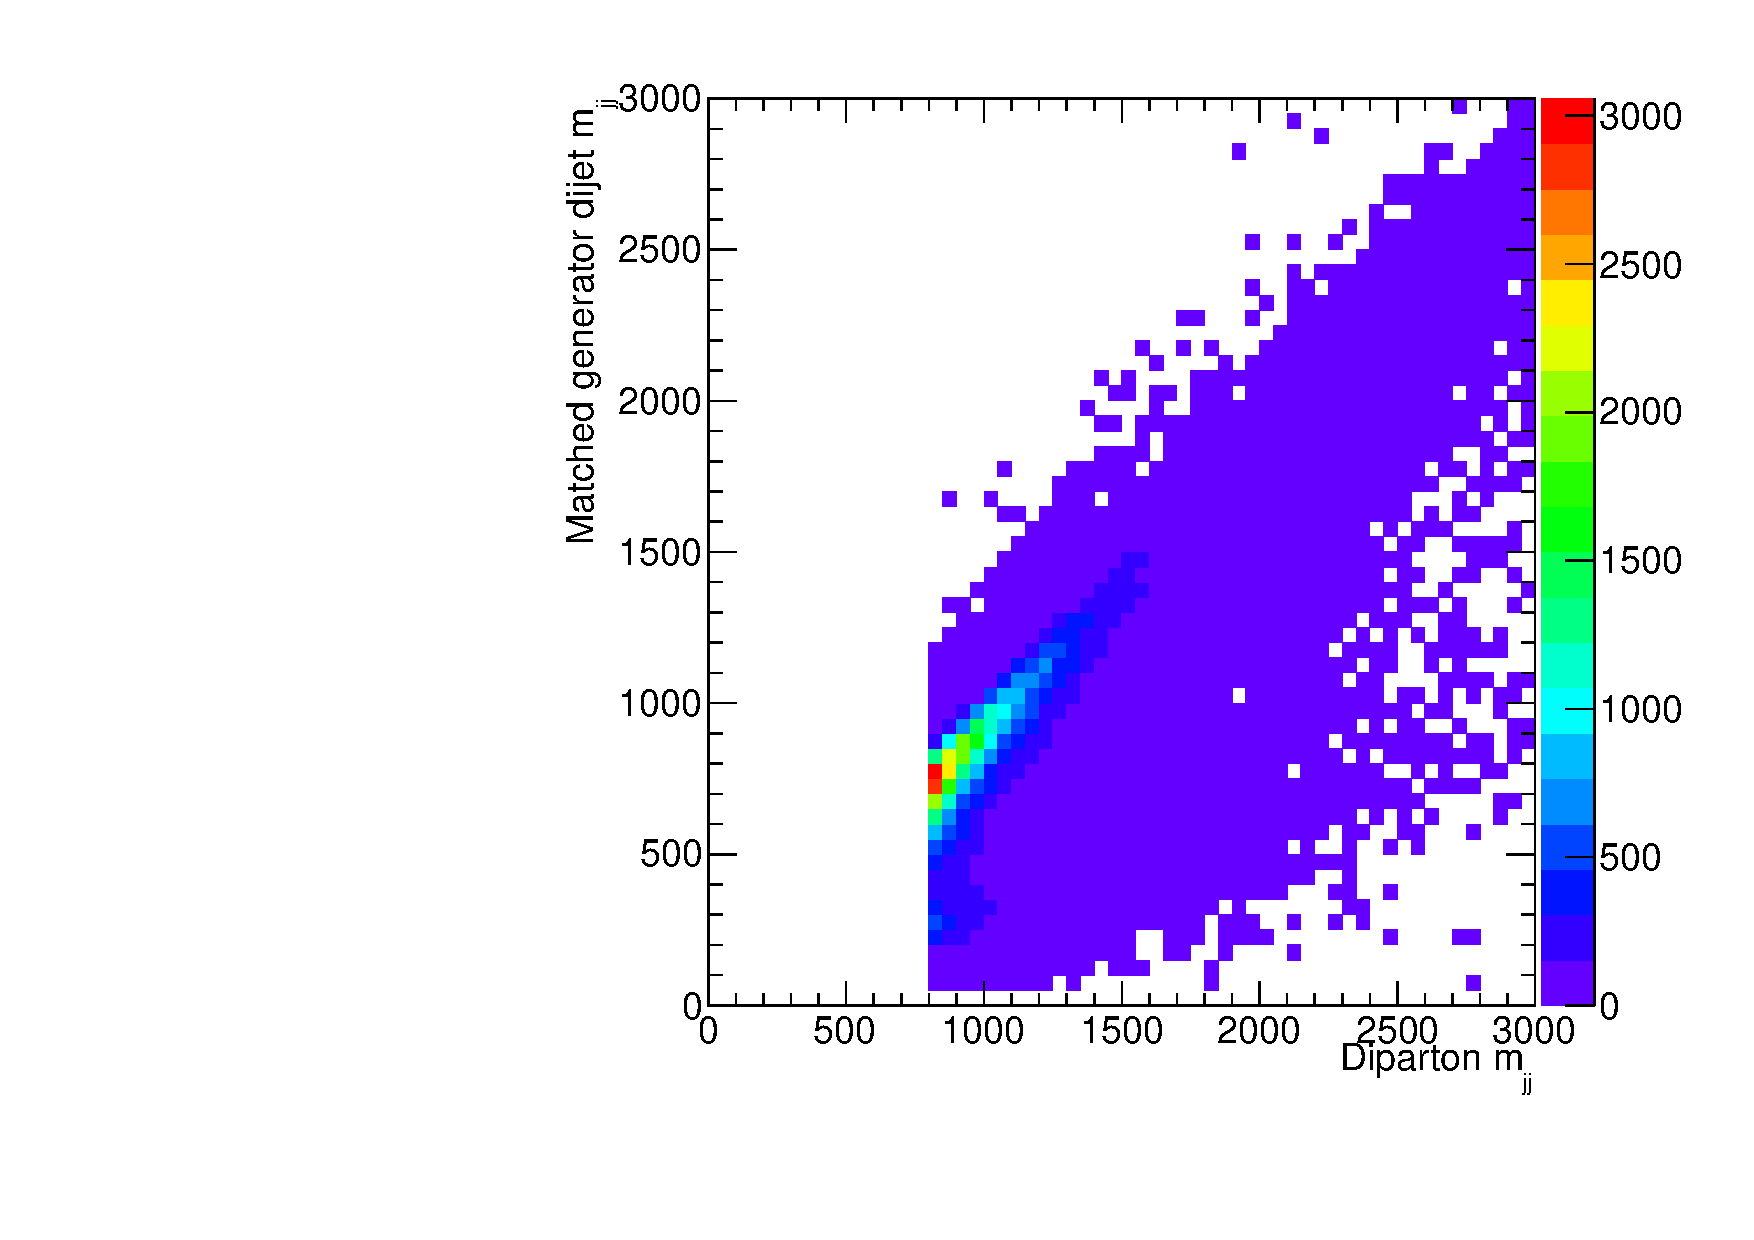
\includegraphics[width=0.40\linewidth]{Chapter07/QCDVBFSamples/Migrations/Images/SelDiParton_MatchedGenJet_Mjj.pdf}}\\
\caption[]{Plots for relevant variables of the selected di-parton against its matched dijet. On plot a) lead parton \pt b) sub-leading parton \pt c) lead parton $\eta$ d) sub-lead parton $\eta$ e) di-parton $\Delta\eta$ d) di-parton $m_{jj}$}
\label{FIGURE:RunIIPreparation_VariablesPartonVsGenJet}
\end{figure}

On plots \ref{FIGURE:RunIIPreparation_VariablesPartonVsGenJet} a), b) and f) we can see two populations. In the parton \pt plots they are along the diagonal and and along the line of generator jet \pt equal to zero and in the $m_{jj}$ plot along the diagonal and along the line of $y=x/2$.  This is due to the fact that at parton level the partons are perfectly matched in energy and momentum but if they are matched to only one correct generator jet and second jet with \pt close to zero, the system will have half the energy of the correctly assigned events.

We can now calculate the event migrations from events that did not pass will not pass the parton event selection but could have passed the generator level selection. This effect can be from jet dispersion or overlap, and clustering artefacts. Let's first consider the migrations on each variable separately, lead jet \pt (eq. \ref{EQUATION:RunIIPreparation_SigleVariableMigrationLeadPt}), sub-lead jet \pt (eq. \ref{EQUATION:RunIIPreparation_SigleVariableMigrationSubleadPt}) and dijet $m_{jj}$ (eq. \ref{EQUATION:RunIIPreparation_SigleVariableMigrationMjj}).

\small
\begin{equation}
\label{EQUATION:RunIIPreparation_SigleVariableMigrationLeadPt}
\frac{p_{T}^{Parton}<30 \wedge p_{T}^{GenJet} \geq 40}{p_{T}^{GenJet} \geq 40}=0.27\% \pm 0.04\%
\end{equation}

\begin{equation}
\label{EQUATION:RunIIPreparation_SigleVariableMigrationSubleadPt}
\frac{p_{T}^{Parton}<30 \wedge p_{T}^{GenJet} \geq 40}{p_{T}^{GenJet} \geq 40}=0.56\% \pm 0.08\%
\end{equation}

\begin{equation}
\label{EQUATION:RunIIPreparation_SigleVariableMigrationMjj}
\frac{m_{jj}^{Parton}<800 \wedge m_{jj}^{GenJet} \geq 1000}{m_{jj}^{GenJet} \geq 800}=0.13\% \pm 0.04\%
\end{equation}
\normalsize

Now we can consider the migrations of events over all variables simultaneously in equation \ref{EQUATION:RunIIPreparation_All}.

\small
\begin{equation}
\label{EQUATION:RunIIPreparation_All}
\frac{(p_{T}^{GenJet}>40 \wedge m_{jj}^{GenJet}>1000) \wedge (p_{T}^{Parton}<30 \vee m_{jj}^{Parton}<800)}{p_{T}^{GenJet}>40 \cup m_{jj}^{GenJet}>1000} = 0.23\% \pm 0.13\%
\end{equation}
\normalsize

We can that that the global migrations of events from below the selected parton level cuts to above the selected generator cuts are of $0.23\% \pm 0.13\%$ of the total number events passing the generator filter. This is an acceptable value which should not bias in any relevant way the physics usage of this sample.

%%%%%%%%%%%%%%%%%%%%%%%%%%%%%%%%%%%%%%%%%%%%%%%%%%%%%%%%%%%%%%%%%%%%%%%%%%%%%%%%%%%%%%%
%%% SUBSECTION
%%%%%%%%%%%%%%%%%%%%%%%%%%%%%%%%%%%%%%%%%%%%%%%%%%%%%%%%%%%%%%%%%%%%%%%%%%%%%%%%%%%%%%%
\subsection{Summary}
\label{SUBSECTION:RunIIPreparation_Summary}

%Status: DONE

The production on new \gls{QCD} \gls{MC} event sample with VBF characteristics was studied and all objectives were achieved. We propose the use as MadGraph as the event generator, configured to produce proton-proton to two, three or four outgoing partons where this partons can be gluons or quarks except the top quark. At the stage we filter the events only accepting those that have at least one di-parton with $m_{jj}>800\,\GeV$ where each parton has at least $30\,\GeV$ and is contained inside the detector acceptance of $|\eta|<5.0|$. This process has a cross section of $1.029 \times 10^7 \pm 1.614 \times 10^4 \,\pico\barn$. 

We proceed with event hadronization using Pythia 8 event generator with MLM jet matching scheme as traditionally done in the \gls{CMS} experiment. We estimate this step to have an efficiency of $9.45\% \pm 0.03\%$ which leads cross section of $9.718 \time 10^5 \pm 2.903 \time 10^3\,\pico\barn$. From those events, we only keep the ones containing at least one generator dijet passing $\Delta\eta > 3.0$, $m_{jj} > 1000\,\GeV$ where both jets pass $\pt > 40\,\GeV$ and $|\eta|<4.8$. We split those event into 2 sub-samples according if the dijet passing all cuts is below (sub-sample A) of above $\Delta\phi=2.15$ (sub-sample B). The filter efficiency for sub-sample A is $2.938 \times 10^{-1} \pm 4.67 \time 10^{-4}$ and it is aimed to have $1\,\femto\barn$ of equivalent integrated luminosity. Sub-ample B filter efficiency is $1.125 \time 10^{-1} \pm 9.13 \time 10^{-4}$ and will have $0.1-1.0\,\femto\barn$ of equivalent integrated luminosity depending on available resources. The overlap between the two sub-samples has been estimated to be of $3.95\% \pm 0.14\%$ thus requiring care in combining them.

Migrations from events below the parton level cuts to about the generator level cuts have been determined to be $0.23\% \pm 0.13\%$ of the total number of events passing the generator filters.

The MadGraph code for event generation have been approved by the \gls{CMS} \gls{MC} production team. The additional code necessary for the generator level filtering has been queued for integration in the experiment software. Final approval of this sample production is under way. 

%TODO: Update if sample is approved.
